\ifdefined\COMPLETE
\else
    \input{./preambule-sacha-utf8.ltx}
    \begin{document}
\fi


\setcounter{section}{0}

\vspace*{-2cm} 

\part{Fonction numérique de la variable réelle}

\section{Généralités}

\subsection{Définitions}

\subsubsection{Fonctions}

\begin{tabular}{ll}
\begin{minipage}{4cm}
\begin{tabular}{llll}
\hspace{-.5cm} Soit $f:$ & $ \R$ &  $\rightarrow$ & $\R$ \\
& $x$ & $\mapsto$ & \hspace*{-.5cm}$\underbrace{f(x)}_{\textrm{image de} x}$ \\
\end{tabular}
\end{minipage}
&
\begin{minipage}{11cm}
$f$ est une fonction numérique de la variable réelle si et seulement si :

\textbf{Tout élément de $\mathbf{\R}$ a au plus une image dans $\mathbf{\R}$.} \\
\end{minipage}
\end{tabular}

\vspace*{.3cm}

\textbf{Remarques :}

\begin{itemize}

\item[*]Vocabulaire : "Au plus une" veut dire, soit une, soit aucune. 

\item[*] $f$ est une fonction et $f(x)$ un nombre réel.

\item[*] \textbf{Attention :} $f$ est une fonction $\neq$ $f(x)$ est un nombre réel.
\end{itemize}

\subsubsection{Ensemble de définition d'une fonction}

\begin{tabular}{lllll}
\hspace{-.3cm} Soit $f:$ & $\R$ & $\longrightarrow$ & $\R$ & une fonction. \\
& $x$ & $\longmapsto$ & $f(x)$ & \\
\end{tabular}

\vspace*{.5cm}

L'ensemble de définition de $f$, noté $D_f$, est l'ensemble des éléments de $\mathbf{\R}$ \\ qui ont une image dans $\mathbf{\R}$.

\vspace*{.3cm}

\textbf{Exemple n°1} 

\begin{tabular}{llll}
\hspace{-.3cm} Soit $f:$ & $\R$ & $\longrightarrow$ & $\R$ \\
& $x$ & $\longmapsto$ & $f(x) = x^2 - 2x - 3$. \\
\end{tabular}

\vspace*{.3cm}

On dit que $f$ est une \textbf{fonction polynôme}. \\

On a $D_f = \R$. \\

\textbf{Exemple n°2} 

\begin{tabular}{llll}
\hspace{-.3cm} Soit $f:$ & $\R$ & $\longrightarrow$ & $\R$ \\
& $x$ & $\longmapsto$ & $f(x) = \dfrac{1}{x^2 - 2x - 3}$. \\
\end{tabular}

\vspace*{.3cm}

On dit que $f$ est une \textbf{fonction rationnelle}. \\

Il ne faut pas que $x^2 - 2x - 3 = 0 \Longleftrightarrow x = -1$ ou $x = 3$. \\

D'où $D_f = \R \setminus \lb -1 \; ; \; 3\rb = \left]-\infty \; ; \; -1\right[ \cup \left]-1 \; ; \; 3\right[ \cup \left] 3 \; ; \; +\infty\right[$.

\vspace*{.3cm}

\textbf{Exemple n°3} 

\begin{tabular}{llll}
\hspace{-.3cm} Soit $f:$ & $\R$ & $\longrightarrow$ & $\R$ \\
& $x$ & $\longmapsto$ & $f(x) = \sqrt{x^2 - 2x - 3}$. \\
\end{tabular}

\vspace*{.3cm}

On dit que $f$ est une \textbf{fonction irrationnelle}. \\

\begin{tabular}{ll}
\hspace*{-.3cm}
\begin{minipage}{5cm}
Il faut que $x^2 - 2x - 3 \geqslant 0$. \\

D'où $D_f = \left]-\infty \; ; \; -1\right[ \cup \left] 3 \; ; \; +\infty\right[$.
\end{minipage}
&
\begin{minipage}{10cm}
\begin{tikzpicture}
\tkzTabInit[lgt=4,espcl=2]
{ $x$               /1,
$x^2 - 2x - 3$     /1}
{$ - \infty $ , $-1$, $3$, $+ \infty $}
\tkzTabLine{ , + , z , - , z , + , }
\end{tikzpicture}
\end{minipage}
\end{tabular}

\vspace*{-5cm}

\newpage

\subsubsection{Représentation graphique d'une fonction}

\begin{tabular}{lllll}
\hspace{-.3cm} Soit $f:$ & $\R$ & $\longrightarrow$ & $\R$ & une fonction. \\
& $x$ & $\longmapsto$ & $f(x)$ & \\
\end{tabular}

\vspace*{.3cm}

Soit $\left(O \; ; \; \overrightarrow{i} \; ; \; \overrightarrow{j}\right)$ un repère. \\ La représentation graphique de $f$, notée $C_f$ est l'ensemble des point $M\left(x \; ; \; f\left(x\right)\right)$, avec $x \in D_f$. \\

\textbf{Exemple n°1} \\

\begin{tabular}{llll}
\hspace{-.3cm} Soit $f:$ & $\R$ & $\longrightarrow$ & $\R$ \\
& $x$ & $\longmapsto$ & $f(x) = x^2 - 2x - 3$. \\
\end{tabular}

\vspace*{.3cm}

On a $D_f = \R = \left]-\infty \; ; \; +\infty\right[$. \\

\begin{tikzpicture}[line cap=round,line join=round,>=triangle 45,x=1.0cm,y=1.0cm]
\draw[->,color=black] (-4.3,0) -- (6.28,0);
\foreach \x in {-4,-3,-2,-1,1,2,3,4,5,6}
\draw[shift={(\x,0)},color=black] (0pt,2pt) -- (0pt,-2pt) node[below] {\footnotesize $\x$};
\draw[->,color=black] (0,-5.32) -- (0,6.3);
\foreach \y in {-5,-4,-3,-2,-1,1,2,3,4,5,6}
\draw[shift={(0,\y)},color=black] (2pt,0pt) -- (-2pt,0pt) node[left] {\footnotesize $\y$};
\draw[color=black] (0pt,-10pt) node[right] {\footnotesize $0$};
\clip(-4.3,-5.32) rectangle (6.28,6.3);
\draw [samples=50,rotate around={0:(1,-4)},xshift=1cm,yshift=-4cm,domain=-5.0:5.0)] plot (\x,{(\x)^2/2/0.5});
\begin{scriptsize}
\draw [fill=black] (-2,5) circle (1.0pt);
\draw [fill=black] (-1,0) circle (1.0pt);
\draw [fill=black] (0,-3) circle (1.0pt);
\draw [fill=black] (1,-4) circle (1.0pt);
\draw [fill=black] (2,-3) circle (1.0pt);
\draw [fill=black] (3,0) circle (1.0pt);
\draw [fill=black] (4,5) circle (1.0pt);
\end{scriptsize}

\begin{pgfonlayer}{background}   
\draw[step=1mm,ultra thin,AntiqueWhite!10] (-4.3,-5.32) grid (6.28,6.3);
\draw[step=5mm,very thin,AntiqueWhite!30]  (-4.3,-5.32) grid (6.28,6.3);
\draw[step=1cm,very thin,AntiqueWhite!50]  (-4.3,-5.32) grid (6.28,6.3);
\draw[step=5cm,thin,AntiqueWhite]          (-4.3,-5.32) grid (6.28,6.3);
\end{pgfonlayer}

\end{tikzpicture}

\vspace*{.3cm}

$C_f$ est une parabole. \\

$f$ est continue sur $\left]-\infty \; ; \; +\infty\right[$. 

\newpage

\textbf{Exemple n°2} \\

\begin{tabular}{llll}
\hspace{-.3cm} Soit $f:$ & $ \R$ & $ \rightarrow$ & $ \R$ \\
& $x$ & $\mapsto$ & $f(x) =\dfrac{x-1}{x+1}$ \\
\end{tabular}

\vspace*{.3cm}

Il ne faut pas que $x+1=0$, donc que $x=-1$. \\

D'où $D_f = \R \setminus \lb -1 \rb = \left]-\infty,-1\right[\cup\left]-1, +\infty\right[$ \\

\begin{tikzpicture}[line cap=round,line join=round,>=triangle 45,x=1.0cm,y=1.0cm]
\draw[->] (-8.84,0) -- (8.96,0);
\foreach \x in {-8,-7,-6,-5,-4,-3,-2,-1,1,2,3,4,5,6,7,8}
\draw[shift={(\x,0)}] (0pt,2pt) -- (0pt,-2pt) node[below] {\footnotesize $\x$};
\draw[->] (0,-7.72) -- (0,6.54);
\foreach \y in {-7,-6,-5,-4,-3,-2,-1,1,2,3,4,5,6}
\draw[shift={(0,\y)}] (2pt,0pt) -- (-2pt,0pt) node[left] {\footnotesize $\y$};
\draw[color=black] (0pt,-10pt) node[right] {\footnotesize $0$};
\clip(-8.84,-7.72) rectangle (8.96,6.54);
\draw[smooth,samples=100,domain=-8.85:-1.1] plot(\x,{((\x)-1)/((\x)+1)});
\draw[smooth,samples=100,domain=-.9:8.96] plot(\x,{((\x)-1)/((\x)+1)});
\draw [color=red] (-1,-7.72) -- (-1,6.54);
\draw [color=red,domain=-8.84:8.96] plot(\x,{(--1-0*\x)/1});

\begin{pgfonlayer}{background}   
\draw[step=1mm,ultra thin,AntiqueWhite!10] (-8.84,-7.72) grid (8.96,6.54);
\draw[step=5mm,very thin,AntiqueWhite!30]  (-8.84,-7.72) grid (8.96,6.54);
\draw[step=1cm,very thin,AntiqueWhite!50]  (-8.84,-7.72) grid (8.96,6.54);
\draw[step=5cm,thin,AntiqueWhite]          (-8.84,-7.72) grid (8.96,6.54);
\end{pgfonlayer}

\end{tikzpicture}

\vspace*{.3cm}

$C_f$ est une hyperbole. \\

$f$ est continue sur $\left]-\infty \; ; \; -1\right[$. \\
$f$ est continue sur $\left]-1 \; ; \; +\infty\right[$. 

\newpage

\textbf{Exemple n°3} \\

\begin{tabular}{llll}
\hspace{-.3cm} Soit $f:$ & $ \R $ & $\rightarrow$ & $\R$ \\
& $x$ & $\mapsto$ & $f(x) = -1 + \sqrt{x+4}$ \\
\end{tabular}

\vspace*{.3cm}

Il faut que $x + 4 \geqslant 0 \Longleftrightarrow x \geqslant -4$. \\

On a donc $D_f = \left[-4 \; ; \; +\infty\right[$. \\

\begin{tikzpicture}[line cap=round,line join=round,>=triangle 45,x=1.0cm,y=1.0cm]
\draw[->,] (-4.3,0) -- (12.74,0);
\foreach \x in {-4,-3,-2,-1,1,2,3,4,5,6,7,8,9,10,11,12}
\draw[shift={(\x,0)}] (0pt,2pt) -- (0pt,-2pt) node[below] {\footnotesize $\x$};
\draw[->] (0,-4.5) -- (0,6.3);
\foreach \y in {-4,-3,-2,-1,1,2,3,4,5,6}
\draw[shift={(0,\y)}] (2pt,0pt) -- (-2pt,0pt) node[left] {\footnotesize $\y$};
\draw[] (0pt,-10pt) node[right] {\footnotesize $0$};
\clip(-4.3,-4.5) rectangle (12.74,6.3);
\draw[smooth,samples=100,domain=-4:12.75] plot(\x,{0-1+sqrt((\x)+4)});
\begin{scriptsize}
\draw (-4,-1)-- ++(-1.0pt,-1.0pt) -- ++(2.0pt,2.0pt) ++(-2.0pt,0) -- ++(2.0pt,-2.0pt);
\draw (-3,0) -- ++(-1.0pt,-1.0pt) -- ++(2.0pt,2.0pt) ++(-2.0pt,0) -- ++(2.0pt,-2.0pt);
\draw (0,1)  -- ++(-1.0pt,-1.0pt) -- ++(2.0pt,2.0pt) ++(-2.0pt,0) -- ++(2.0pt,-2.0pt);
\draw (5,2)  -- ++(-1.0pt,-1.0pt) -- ++(2.0pt,2.0pt) ++(-2.0pt,0) -- ++(2.0pt,-2.0pt);
\draw (12,3) -- ++(-1.0pt,-1.0pt) -- ++(2.0pt,2.0pt) ++(-2.0pt,0) -- ++(2.0pt,-2.0pt);
\end{scriptsize}

\begin{pgfonlayer}{background}   
\draw[step=1mm,ultra thin,AntiqueWhite!10] (-4.3,-4.5) grid (12.74,6.3);
\draw[step=5mm,very thin,AntiqueWhite!30]  (-4.3,-4.5) grid (12.74,6.3);
\draw[step=1cm,very thin,AntiqueWhite!50]  (-4.3,-4.5) grid (12.74,6.3);
\draw[step=5cm,thin,AntiqueWhite]          (-4.3,-4.5) grid (12.74,6.3);
\end{pgfonlayer}

\end{tikzpicture}

\vspace*{.3cm}

$C_f$ est une demi-parabole. \\

$f$ est continue sur $\left[-4 \; ; \; +\infty\right[$.

\newpage

\subsection{Fonction continue sur un intervalle}

\subsubsection{Définition}

\begin{tabular}{lllll}
\hspace{-.3cm} Soit $f:$ & $\R$ & $\longrightarrow$ & $\R$ & une fonction. \\
& $x$ & $\longmapsto$ & $f(x)$ & \\
\end{tabular}

\vspace*{.3cm}

Soit $I$ un intervalle inclus dans $D_f$. Soit $C_f$ la représentation graphique de $f$ dans un repère $\left(O \; ; \; \overrightarrow{i} \; ; \; \overrightarrow{j}\right)$. \\
Dire que $f$ est continue sur $I$, c'est dire que l'on peut tracer $C_f$ sur $I$ sans lever le crayon.

\subsubsection{Exemple \no 1}

\begin{tabular}{llllllll}
\hspace{-.3cm} Soit la fonction $f$ : & $\R$ & $\longrightarrow$ & $\R$ & & & & \\
& $x$ & $\longmapsto$ & $f\left(x\right)$ & $ = $ & $ x + 2$ & si & $x \in \left]-\infty \; ; \; -2\right[$ \\
& & & & $=$ & $-x - 2$ &  si & $x \in \left]-2 \; ; \; 2\right[$ \\
& & & & $=$ & $x + 2$ &  si & $x \in \left]2 \; ; \; +\infty\right[$ \\
& & & $f\left(-2\right)$ & $=$ & $0$ \\
& & & $f\left(2\right)$ & $=$ & $0$ \\
\end{tabular}

\vspace*{.3cm}

On a $D_f = \R$. \\

\begin{tikzpicture}[line cap=round,line join=round,>=triangle 45,x=1.0cm,y=1.0cm=scala=.8]
\draw[->,color=black] (-6.67,0) -- (6.6,0);
\foreach \x in {-6,-5,-4,-3,-2,-1,1,2,3,4,5,6}
\draw[shift={(\x,0)},color=black] (0pt,2pt) -- (0pt,-2pt) node[below] {\footnotesize $\x$};
\draw[->,color=black] (0,-5.69) -- (0,8.25);
\foreach \y in {-5,-4,-3,-2,-1,1,2,3,4,5,6,7,8}
\draw[shift={(0,\y)},color=black] (2pt,0pt) -- (-2pt,0pt) node[left] {\footnotesize $\y$};
\draw[color=black] (0pt,-10pt) node[right] {\footnotesize $0$};
\clip(-6.67,-5.69) rectangle (6.6,8.25);
\draw [domain=-6.667491653245479:-2.0] plot(\x,{(-4-2*\x)/-2});
\draw (-2,0)-- (2,-4);
\draw [domain=2.0:6.596313424673678] plot(\x,{(--4--2*\x)/2});
\begin{scriptsize}
\draw[color=black] (-3.17,-0.64) node {};
\draw[color=black] (-0.16,-2.06) node {};
\draw[color=black] (3.27,4.94) node {};
\end{scriptsize}
\begin{pgfonlayer}{background}   
\draw[step=1mm,ultra thin,AntiqueWhite!10] (-6.67,-5.69) grid (6.6,8.25);
\draw[step=5mm,very thin,AntiqueWhite!30]  (-6.67,-5.69) grid (6.6,8.25);
\draw[step=1cm,very thin,AntiqueWhite!50]  (-6.67,-5.69) grid (6.6,8.25);
\draw[step=5cm,thin,AntiqueWhite]          (-6.67,-5.69) grid (6.6,8.25);
\end{pgfonlayer} 
\end{tikzpicture}

\vspace*{.3cm}

$f$ n'est pas continue sur $\R$ mais $f$ est continue sur $\left]-\infty \; ; \; 2\right[$ et $f$ est continue sur $\left]2 \; ; \; +\infty\right[$.

\vspace*{-5cm}

\newpage

\subsubsection{Exemple \no 2}

\begin{tabular}{llllllll}
\hspace{-.3cm} Soit la fonction $f$ : & $\R$ & $\longrightarrow$ & $\R$ & & & & \\
& $x$ & $\longmapsto$ & $f\left(x\right)$ & $ = $ & $ \dfrac{2x - 8}{x-3}$ & si & $x \in \left]-\infty \; ; \; 2\right[$ \vspace*{.3cm} \\
& & & & $=$ & $-x^2 + 6x - 4$ &  si & $x \in \left]2 \; ; \; 5\right[$ \vspace*{.3cm} \\
& & & & $=$ & $\dfrac{2x - 8}{x-3}$ &  si & $x \in \left]5 \; ; \; +\infty\right[$ \vspace*{.3cm} \\
& & et & $f(2)$ & $ = $ & $4$ & & \\
& & et & $f(5)$ & $ = $ & $1$ & & \\
\end{tabular}

On a $D_f = \R$. \\

\definecolor{wwqqzz}{rgb}{0.4,0,0.6}
\definecolor{uuuuuu}{rgb}{0.27,0.27,0.27}
\definecolor{qqccqq}{rgb}{0,0.8,0}
\definecolor{ffqqqq}{rgb}{1,0,0}
\begin{tikzpicture}[line cap=round,line join=round,>=triangle 45,x=1.0cm,y=1.0cm, scale=.92]
\draw[->,color=black] (-5.33,0) -- (11.35,0);
\foreach \x in {-5,-4,-3,-2,-1,1,2,3,4,5,6,7,8,9,10,11}
\draw[shift={(\x,0)},color=black] (0pt,2pt) -- (0pt,-2pt) node[below] {\footnotesize $\x$};
\draw[->,color=black] (0,-6.2) -- (0,12.91);
\foreach \y in {-6,-5,-4,-3,-2,-1,1,2,3,4,5,6,7,8,9,10,11,12}
\draw[shift={(0,\y)},color=black] (2pt,0pt) -- (-2pt,0pt) node[left] {\footnotesize $\y$};
\draw[color=black] (0pt,-10pt) node[right] {\footnotesize $0$};
\clip(-5.33,-6.2) rectangle (11.35,12.91);
\draw[color=ffqqqq,smooth,samples=100,domain=3.1:11] plot(\x,{(2*(\x)-8)/((\x)-3)});
\draw[color=ffqqqq] plot[raw gnuplot, id=func0] function{set samples 100; set xrange [2.1:4.9]; plot -x**(2)+6*x-4};
\draw[color=ffqqqq,smooth,samples=100,domain=-5.3:2.9] plot(\x,{(2*(\x)-8)/((\x)-3)});
\draw[smooth,samples=100,domain=2.0:2.9] plot(\x,{(2*(\x)-8)/((\x)-3)});
\draw[smooth,samples=100,domain=3.01:5.0] plot(\x,{(2*(\x)-8)/((\x)-3)});
\draw [smooth,samples=100,domain=-1:2] plot(\x,{(-1)*(\x)*(\x)  +6*(\x)-4});
\draw [color=red,smooth,samples=100,domain=2:5] plot(\x,{(-1)*(\x)*(\x)  +6*(\x)-4});
\draw [smooth,samples=100,domain=5:8] plot(\x,{(-1)*(\x)*(\x)  +6*(\x)-4});
\draw [color=qqccqq] (3,-6.2) -- (3,12.91);
\draw [color=wwqqzz,domain=-5.33:11.35] plot(\x,{(-0--2*\x)/1});
\draw [color=wwqqzz,domain=-5.33:11.35] plot(\x,{(--21-4*\x)/1});
\draw [color=qqccqq] (11.5,2) -- (-5.5,2);
\begin{scriptsize}
\draw[color=ffqqqq] (-5.12,2.08) node {};
\draw[color=ffqqqq] (2.35,3.89) node {};
\draw[color=ffqqqq] (5.39,0.86) node {};
\draw[color=black] (2.33,3.84) node {};
\draw[color=black] (3.58,-5.86) node {};
\draw[color=black] (-0.03,-5.86) node {};
\draw[color=black] (5.36,0.72) node {};
\draw[color=qqccqq] (3.27,12.73) node {};
\draw [fill=uuuuuu] (2,4) circle (1.5pt);
\draw[color=uuuuuu] (1.67,4.28) node {$A$};
\draw [fill=uuuuuu] (5,1) circle (1.5pt);
\draw[color=uuuuuu] (5.15,1.4) node {$B$};
\draw[color=wwqqzz] (5.96,12.73) node {};
\draw[color=wwqqzz] (2.38,12.73) node {};
\end{scriptsize}
\begin{pgfonlayer}{background}   
\draw[step=1mm,ultra thin,AntiqueWhite!10] (-5.33,-6.2) grid (11.35,12.91);
\draw[step=5mm,very thin,AntiqueWhite!30]  (-5.33,-6.2) grid (11.35,12.91);
\draw[step=1cm,very thin,AntiqueWhite!50]  (-5.33,-6.2) grid (11.35,12.91);
\draw[step=5cm,thin,AntiqueWhite]          (-5.33,-6.2) grid (11.35,12.91);
\end{pgfonlayer} 
\end{tikzpicture}

\subsubsection{Exercice \no 1}

Le tarif en euros pratiqué à la journée par une commune pour l'accueil des enfants selon le quotient familial est associé à une fonction $f$. \\

\begin{tabular}{llllllll}
\hspace*{-.3cm} $f:$ & $\left[0 \; ; \; +\infty\right[$ & $\longrightarrow$ & $\R$ \\
& $\; \; \; \; \; \; \; \; x$ & $\longmapsto$ & $f(x)$ & $=$ & $3$ & si & $0 \leqslant x < 400$ \\
& & & & $=$ & $6$ & si & $400 \leqslant x < 600$ \\
& & & & $=$ & $8$ & si & $600 \leqslant x < 1200$ \\
& & & & $=$ & $10$ & si & $x \geqslant 1200$ \\
\end{tabular}

\vspace*{.3cm}

\definecolor{qqwwtt}{rgb}{0,0.4,0.2}
\begin{tikzpicture}[line cap=round,line join=round,>=triangle 45,x=1.0cm,y=1.0cm]
\draw[->] (-0.56,0) -- (14.52,0);
\foreach \x in {,1,2,3,4,5,6,7,8,9,10,11,12,13,14}
\draw[shift={(\x,0)}] (0pt,2pt) -- (0pt,-2pt) ; % node[below] {\footnotesize $\x$};
\draw (2,0) node[below] {\footnotesize $200$};
\draw (4,0) node[below] {\footnotesize $400$};
\draw (6,0) node[below] {\footnotesize $600$};
\draw (8,0) node[below] {\footnotesize $800$};
\draw (10,0) node[below] {\footnotesize $1000$};
\draw (12,0) node[below] {\footnotesize $1200$};
\draw[->] (0,-0.98) -- (0,11.42);
\foreach \y in {,1,2,3,4,5,6,7,8,9,10,11}
\draw[shift={(0,\y)}] (2pt,0pt) -- (-2pt,0pt) node[left] {\footnotesize $\y$};
\draw[] (-.2,0) node[below] {\footnotesize $0$};
\clip(-0.56,-0.98) rectangle (14.52,11.42);
\draw [color=DarkGreen] (0,3)-- (4,3);
\draw [color=DarkGreen] (4,6)-- (6,6);
\draw [color=DarkGreen] (6,8)-- (12,8);
\draw [color=DarkGreen] (12,10)-- (15,10);
\begin{scriptsize}
\draw [fill=DarkGreen] (0,3) circle (1.5pt);
\draw [color=DarkGreen] (4,3)-- ++(0pt,0pt) -- ++(2.5pt,2.5pt)   ++(0pt,-5pt) -- ++(-2.5pt,2.5pt);
\draw [fill=DarkGreen] (4,6) circle (1.0pt);
\draw [color=DarkGreen] (6,6)-- ++(0pt,0pt) -- ++(2.5pt,2.5pt)   ++(0pt,-5pt) -- ++(-2.5pt,2.5pt);
\draw [fill=DarkGreen] (6,8) circle (1.0pt);
\draw [color=DarkGreen] (12,8)-- ++(0pt,0pt) -- ++(2.5pt,2.5pt)   ++(0pt,-5pt) -- ++(-2.5pt,2.5pt);
\draw [fill=DarkGreen] (12,10) circle (1.0pt);
\end{scriptsize}

\begin{pgfonlayer}{background}   
\draw[step=1mm,ultra thin,AntiqueWhite!10] (-0.56,-0.98) grid (14.52,11.42);
\draw[step=5mm,very thin,AntiqueWhite!30]  (-0.56,-0.98) grid (14.52,11.42);
\draw[step=1cm,very thin,AntiqueWhite!50]  (-0.56,-0.98) grid (14.52,11.42);
\draw[step=5cm,thin,AntiqueWhite]          (-0.56,-0.98) grid (14.52,11.42);
\end{pgfonlayer}

\end{tikzpicture}

\vspace*{.3cm}

$f$ est une fonction escalier. \\

$f$ n'est pas continue sur $\left[0 \; ; \; +\infty\right[$.

\newpage

\subsubsection{Exercice \no 2}

À 8h45, Sylvain part à pied d'une ville $A$ pour aller dans une ville $B$ située à $20$km de $A$. \\
Son parcours est associé à la fonction $f$ suivante :

\begin{tabular}{llllllll}
\hspace*{-.3cm} $f:$ & $\left[0 \; ; \; 300\right]$ & $\longrightarrow$ & $\R$ \\
& $\; \; \; \; \; \; \; \; x$ & $\longmapsto$ & $f(x)$ & $=$ & $\dfrac{1}{15}$ & si & $0 \leqslant x \leqslant 150$ \vspace*{.3cm} \\
& & & & $=$ & $10$ & si & $150 \leqslant x \geqslant 180$ \\
& & & & $=$ & $\dfrac{1}{12}x - 5$ & si & $180 \leqslant x \geqslant 300$ \\
\end{tabular}

\vspace*{.3cm}

\begin{tikzpicture}[line cap=round,line join=round,>=triangle 45,x=1.0cm,y=1.0cm, scale=0.7]
\draw[->] (-0.6,0) -- (20.72,0);
% Attention de ne pas mettre de cas vide (ie ,,) dans cette liste 
\foreach \x in {1,2,3,4,5,6,7,8,9,10,11,12,13,14,15,16,17,18,19,20}
{% ------- attention aux accollades ----------
    \pgfmathsetmacro\ECHL{\x * 15}
    \draw[shift={(\x,0)}] (0pt,2pt) -- (0pt,-2pt) node[below] {\footnotesize $\pgfmathprintnumber{\ECHL}$};
}
\draw[->] (0,-0.96) -- (0,10.75);
\foreach \y in {1,2,3,4,5,6,7,8,9,10}
{\pgfmathsetmacro\ECHL{\y * 2}
\draw[shift={(0,\y)}] (2pt,0pt) -- (-2pt,0pt) node[left] {\footnotesize $\pgfmathprintnumber{\ECHL}$};
}
\draw (0pt,-10pt) node[right] {\footnotesize $0$};
\clip(-0.6,-0.96) rectangle (20.72,10.75);
\draw[color=DarkGreen,smooth,samples=100,domain=0.0:10.0] plot(\x,{0.5*(\x)});
\draw[color=DarkGreen,smooth,samples=100,domain=10.0:12.0] plot(\x,{5});
\draw[color=DarkGreen,smooth,samples=100,domain=12.0:20.0] plot(\x,{5/8*(\x)-5/2});

\begin{pgfonlayer}{background}   
\draw[step=1mm,ultra thin,AntiqueWhite!10] (-0.6,-0.96) grid (20.72,10.75);
\draw[step=5mm,very thin,AntiqueWhite!30]  (-0.6,-0.96) grid (20.72,10.75);
\draw[step=1cm,very thin,AntiqueWhite!50]  (-0.6,-0.96) grid (20.72,10.75);
\draw[step=5cm,thin,AntiqueWhite]          (-0.6,-0.96) grid (20.72,10.75);
\end{pgfonlayer}

\end{tikzpicture}

\vspace*{.3cm}

$f$ est une fonction affine par morceaux. \\

$f$ est continue sur $\left[0 \; ; \; 300\right]$.

\subsubsection{Théorèmes fondamentaux}

\begin{itemize}
\item[•] Toute fonction polynôme est continue sur $\R$. \\
\item[•] Toute fonction rationnelle est continue sur chacun des intervalles de son ensembles de définition. \\

Par exemple, si $f(x) = \dfrac{x+3}{x-5}$, on a $D_f = \R \setminus \lb 5 \rb = \left]-\infty \; ; \; 5\right[ \cup \left]5 \; ; \; +\infty\right[$. \\

$f$ n'est pas continue sur $\R \setminus \lb 5 \rb$, mais $f$ est continue sur $\left]-\infty \; ; \; 5\right[$ et sur $\left]5 \; ; \; +\infty\right[$. 
\end{itemize}

\newpage

\vspace*{-2cm}

\subsection{Fonction dérivable sur un intervalle}

\subsubsection{Fonction dérivable en un point}

\textbf{Exemple n°1} \\

\begin{tabular}{llll}
\hspace{-.3cm} Soit la fonction $f$ : & $\R$ & $\longrightarrow$ & $\R$ \\
& $x$ & $\longmapsto$ & $f\left(x\right) = x^2$ \\
\end{tabular}

On a $D_f = \R$. \\

Montrons que $f$ est dérivable en $x_0 = 5$. On a alors $f(5) = 25$. \\

\begin{tabular}{llll}
$T(h)$ & $=$ & $\dfrac{f(x_0 + h) - f(x_0)}{h}$ & \vspace*{.3cm} \\
& $=$ & $\dfrac{f(5 + h) - f(5)}{h}$ & \vspace*{.3cm} \\
& $=$ & $\dfrac{(5+h)^2 - 25}{h}$ & \vspace*{.3cm} \\
& $=$ & $\dfrac{h^2 + 10h + 25 - 25}{h}$ & \vspace*{.3cm} \\
& $=$ & $\dfrac{h^2 + 10h}{h}$ & \vspace*{.3cm} \\
& $=$ & $\dfrac{h\left(h+ 10\right)}{h}$ & \vspace*{.3cm} \\
& $=$ & $ h + 10$ & si $h \neq 0$ \vspace*{.3cm} \\
\end{tabular}

$\lim\limits_{h \to 0} T(h) = \lim\limits_{h \to 0} (h + 10) = 10$. Donc $f$ est dérivable en $x_0 = 5$ et $f'(5) = 10$. \\

\textbf{Exemple n°2} \\

\begin{tabular}{llll}
\hspace{-.3cm} Soit la fonction $f$ : & $\R$ & $\longrightarrow$ & $\R$ \\
& $x$ & $\longmapsto$ & $f\left(x\right) = \dfrac{1}{x}$ \\
\end{tabular}

On a $D_f = \R \setminus \lb 0 \rb$. \\

Montrons que $f$ est dérivable en $x_0 = 5$. On a alors $f(5) = \dfrac{1}{5}$. \\

\begin{tabular}{llclc}
$T(h)$ & $=$ & $\dfrac{f(x_0 + h) - f(x_0)}{h}$ & $=$ & $\dfrac{f(5 + h) - f(5)}{h}$ \vspace*{.3cm} \\
& $=$ & $\dfrac{ \dfrac{1}{5+h} - \dfrac{1}{5}}{h}$ & $=$ & $\dfrac{\dfrac{5-(5+h)}{5(5+h)}}{h}$ \vspace*{.3cm} \\
& $=$ & $\dfrac{\dfrac{-h}{5(5+h)}}{h}$ & $=$ & $\dfrac{-h}{5(5+h)} \times \dfrac{1}{h}$ \vspace*{.3cm} \\
& $=$ & $\dfrac{-1}{5\left(5+h\right)} \; \; \; \; \; \; \; $ si $h \neq 0$ \\
\end{tabular}

\vspace*{.5cm}

$\lim\limits_{h \to 0} T(h) = \lim\limits_{h \to 0} \dfrac{-1}{5\left(5+h\right)} = \dfrac{-1}{25}$. Donc $f$ est dérivable en $x_0 = 5$ et $f'(5) = -\dfrac{1}{25}$. 

\vspace*{-5cm}

\newpage

\subsubsection{Fonction dérivable sur un intervalle}

\textbf{Exemple n°1} \\

\begin{tabular}{llll}
\hspace{-.3cm} Soit la fonction $f :$ & $\R$ & $\longrightarrow$ & $\R$ \\
& $f$ & $\longmapsto$ & $f(x) = x^2$ \\
\end{tabular}

On a $D_f = \R$. \\

Soit $x_0 \in D_f$. \\

Montrons que $f$ est dérivable en $x_0$. \\

\begin{itemize}
\item[•] Calcul du taux d'accroissement : \vspace*{.3cm}
\\
\begin{tabular}{llll}
$T(h)$ & $=$ & $\dfrac{f(x_0 + h) - f(x_0)}{h}$ & \vspace*{.3cm} \\
& $=$ & $\dfrac{\left(x_0 + h\right)^2 - x_0^2}{h}$ & \vspace*{.3cm} \\
& $=$ & $\dfrac{x_0^2 + 2x_0h + h^2 - x_0^2}{h}$ & \vspace*{.3cm} \\
& $=$ & $\dfrac{2x_0h + h^2}{h}$ & \vspace*{.3cm} \\
& $=$ & $\dfrac{h\left(2x_0 + h\right)}{h}$ & \vspace*{.3cm} \\
& $=$ & $2x_0 + h$ & si $h \neq 0$ \\
\end{tabular} \\
\vspace*{.3cm}

\item[•] Limite du taux d'accroissement : \vspace*{.3cm}

$\lim\limits_{h \to 0} T(h) = \lim\limits_{h \to 0} (2x_0 + h) = 2x_0$ \vspace*{.3cm} \\

Donc $f$ est dérivable en $x_0$ et $f'(x_0) = 2x_0$. \\

\item[•] Fonction dérivée : \\

\begin{tabular}{llllll}
$f' :$ & $\R$ & $\longrightarrow$ & $\R$ & & \\
& $x_0$ & $\longmapsto$ & $f'(x_0)$ & $ = $ & $2x_0$ \\
& $x$ & $\longmapsto$ & $f'(x)$ & $ = $ & $2x$ \\
\end{tabular}
\end{itemize}

\vspace*{.3cm}

On a $D_{f'} = \R$ \\

\newpage

\textbf{Exemple n°2} \\

\begin{tabular}{llll}
\hspace{-.3cm} Soit la fonction $f :$ & $\R$ & $\longrightarrow$ & $\R$ \\
& $f$ & $\longmapsto$ & $f(x) = \dfrac{1}{x} $ \\
\end{tabular}

On a $D_f = \R \setminus \lb 0 \rb $. \\

Soit $x_0 \in D_f$. \\

Montrons que $f$ est dérivable en $x_0$. \\

\begin{itemize}
\item[•] Calcul du taux d'accroissement : \vspace*{.3cm}
\\
\begin{tabular}{llll}
$T(h)$ & $=$ & $\dfrac{f(x_0 + h) - f(x_0)}{h}$ & \vspace*{.3cm} \\
& $=$ & $\dfrac{\dfrac{1}{x_0 + h} - \dfrac{1}{x_0}}{h}$ & \vspace*{.3cm} \\
& $=$ & $\dfrac{\dfrac{x_0-\left(x_0 + h\right)}{x_0\left(x_0 + h\right)}}{h}$ & \vspace*{.3cm} \\
& $=$ & $\dfrac{\dfrac{x_0 - x_0 - h}{x_0\left(x_0 + h\right)}}{h}$ & \vspace*{.3cm} \\
& $=$ & $\dfrac{\dfrac{-h}{x_0\left(x_0 + h\right)}}{h}$ & \vspace*{.3cm} \\
& $=$ & $\dfrac{-h}{x_0\left(x_0 + h\right)} \times \dfrac{1}{h}$ & \vspace*{.3cm} \\
& $=$ & $\dfrac{-1}{x_0\left(x_0 + h\right)}$ & si $h \neq 0$ \\
\end{tabular} \\
\vspace*{.3cm}

\item[•] Limite du taux d'accroissement : \vspace*{.3cm}

$\lim\limits_{h \to 0} T(h) = \lim\limits_{h \to 0} \dfrac{-1}{x_0\left(x_0 + h\right)} = \dfrac{-1}{x_0^2}$ \vspace*{.3cm} \\

Donc $f$ est dérivable en $x_0$ et $f'(x_0) = \dfrac{-1}{x_0^2}$. \\

\item[•] Fonction dérivée : \\

\begin{tabular}{llllll}
$f' :$ & $\R$ & $\longrightarrow$ & $\R$ & & \\
& $x_0$ & $\longmapsto$ & $f'(x_0)$ & $ = $ & $\dfrac{-1}{x_0^2}$ \vspace*{.3cm} \\
& $x$ & $\longmapsto$ & $f'(x)$ & $ = $ & $\dfrac{-1}{x^2}$ \\
\end{tabular}
\end{itemize}

\vspace*{.3cm}

On a $D_{f'} = \R \setminus \lb 0 \rb $.
 
\vspace*{-5cm}

\newpage

\subsubsection{Fonction dérivées de fonctions usuelles}

\vspace*{.3cm}

\begin{tabular}{|c|c|c|}
\hline
& & \\
$f\left(x\right)$ & $f'\left(x\right)$ & $f$ est dérivable sur... \\
& & \\
\hline
& & \\
$x$ & $0$ & $\R = \left]-\infty \; ; \; +\infty\right[$ \\
& & \\
\hline
& & \\
$ax + b$ & $a$ & $\R = \left]-\infty \; ; \; +\infty\right[$ \\
& & \\
\hline
& & \\
$x$ & $1$ & $\R = \left]-\infty \; ; \; +\infty\right[$ \\
& & \\
\hline
& & \\
$x^2$ & $2x$ & $\R = \left]-\infty \; ; \; +\infty\right[$ \\
& & \\
\hline
& & \\
$x^n$ & $nx^{n-1}$ & $\R = \left]-\infty \; ; \; +\infty\right[$ \\
& & \\
\hline
& & \\
$\dfrac{1}{x}$ & $\dfrac{-1}{x^2}$ & $\left]-\infty \; ; \; 0\right[$ ou $\left]0\; ; \; +\infty\right[$ \\
& & \\
\hline
& & \\
$\sqrt{x}$ & $\dfrac{-1}{2\sqrt{x}}$ & $\left]0\; ; \; +\infty\right[$ \\
& & \\
\hline
& & \\
$e^x$ & $e^x$ & $\R = \left]-\infty \; ; \; +\infty\right[$ \\
& & \\
\hline
& & \\
$\ln x$ & $\dfrac{1}{x}$ & $\left]0 \; ; \; +\infty\right[$ \\
& & \\
\hline
\end{tabular}

\vspace*{.3cm}

\textbf{N.B. :} Les fonctions exponentielle, notée $e$ et logarithme népérien, notée $\ln$, seront étudiées plus tard dans le cours.

\newpage

\subsubsection{Formules fondamentales}

Soient $u$ et $v$ deux fonctions définie sur un même intervalle $I$. \\ Soit $\lambda \in \R$. \\

On a :  \\

\begin{itemize}
\item[•] $\left(u + v\right)' = u' + v'$. \\
\item[•] $\left(\lambda u\right)' = \lambda u'$. \\ 
\item[•] $\left(uv\right)' = u'v + uv'$.  \\
\item[•] $\left(u^n\right)' = nu^{n-1}u'$. \\
\item[•] $\left(\dfrac{1}{v}\right)' = \dfrac{-v'}{v^2}$. \\
\item[•] $\left(\dfrac{u}{v}\right)' = \dfrac{u'v - uv'}{v^2}$. \\
\item[•] $\left(\sqrt{u}\right)' = \dfrac{u'}{2\sqrt{u}}$. \\
\item[•] $\left(e^u\right)' = u'e^u$.
\end{itemize}

\subsubsection{Exemple}

\begin{tabular}{llll}
Soit $f:$ & $\R$ & $\longrightarrow$ & $\R$ \\
& $x$ & $\longmapsto$ & $\left(5x - 3\right)^2$ \\
\end{tabular}

\vspace*{.5cm}

Calculer $f'(x)$ de deux façons différentes. \\

\begin{itemize}
\item[•] $f(x) = \left(5x - 3\right)^2 = 25x^2 - 30x + 19$. \\

Donc $f'(x) = 50x - 30$. \\

\item[•] $f(x) = \left(5x - 3\right)^2$. \\

Donc $f'(x) = 2\left(5x - 3\right) \times 5 = 10\left(5x - 3\right) = 50x - 30$.
\end{itemize}

\newpage

\subsubsection{Calculs de dérivées}

\textbf{Exercice n°1} \\

\begin{tabular}{llll}
\hspace{-.3cm} Soit $f:$ & $\R$ & $\longrightarrow$ & $\R$ \\
& $x$ & $\longmapsto$ & $f(x) = \dfrac{4x^2 - 17x+1}{x^2 - 5x + 4}$ \\
\end{tabular}

\vspace*{.3cm}

\begin{tabular}{lll}
\hspace*{-.3cm} Il ne faut pas que $x^2 - 5x + 4 = 0$ & $\Longleftrightarrow$ & $\left(x-1\right)\left(x-4\right) = 0$ \\
& $\Longleftrightarrow$ & $x-1 = 0$ ou $x-4 = 0$ \\
& $\Longleftrightarrow$ & $x = 1$ ou $x=4$ \\
\end{tabular}

\vspace*{.3cm}

Donc $D_f = \R \setminus \lb 1 \; ; \; 4 \rb = \left]-\infty \; ; \; 1 \right[\cup \left]1 \; ; \; 4\right[ \cup \left]4 \; ; \; +\infty\right[$. \\

\begin{tabular}{llll}
\hspace{-.3cm} On pose & $u(x) = 4x^2 - 17x + 1$ & et & $v(x) = x^2 - 5x + 4$ \\
\hspace{-.3cm} D'où & $u'(x) = 8x - 17$ & et & $v'(x) = 2x - 5$ \\
\end{tabular}

On a $f = \dfrac{u}{v}$, donc $f' = \dfrac{u'v - uv'}{v^2}$. \vspace*{.3cm} \\

\begin{tabular}{lll}
\hspace*{-.3cm} Ainsi $\forall x \in D_f, f'(x)$ & $=$ & $\dfrac{\left(8x-17\right)\left(x^2-5x+4\right) - \left(4x^2-17x+1\right)\left(2x-5\right)}{\left(x^2-5x+4\right)^2}$ \vspace*{.3cm} \\
& $=$ & $\dfrac{\left(8x^3 - 40x^2 + 32x - 17x^2 + 85x - 68\right) - \left(8x^3 - 20x^2 - 34x^2 + 85x + 2x - 5\right)}{\left(x^2-5x+4\right)^2}$ \vspace*{.3cm} \\
& $=$ & $\dfrac{8x^2 - 40x^2 + 32x - 17x^2 + 85x - 68 - 8x^3 + 20x^2 + 34x^2 - 85x - 2x + 5}{\left(x^2 - 5x + 4\right)^2}$ \vspace*{.3cm} \\
& $=$ & $\dfrac{-3x^2 + 30x - 63}{\left(x^2 - 5x + 4\right)^2}$ \\
\end{tabular}

\vspace*{.3cm}

Donc $\forall x \in D_f, f'(x) = \dfrac{-3x^2 + 30x - 63}{\left(x^2 - 5x + 4\right)^2}$. \vspace*{.3cm} \\

\begin{tabular}{lll}
\hspace*{-.3cm} On a $f'(x) = 0$ & $\Longleftrightarrow$ & $\dfrac{-3x^2 + 30x - 63}{\left(x^2 - 5x + 4\right)^2} = 0$ \vspace*{.3cm} \\
& $\Longleftrightarrow$ & $-3x^2 + 30x - 63 = 0$ \vspace*{.3cm} \\
& $\Longleftrightarrow$ & $x=3$ ou $x=7$ \\
\end{tabular}

\vspace*{-5cm}

\newpage

\textbf{Exercice n°2} \\

\begin{tabular}{llll}
\hspace{-.3cm} Soit $f:$ & $\R$ & $\longrightarrow$ & $\R$ \\
& $x$ & $\longmapsto$ & $f(x) = \left(3x+2\right)^2\left(2x-5\right)^3$ \\
\end{tabular}

\vspace*{.3cm}

Donc $D_f = \R$. \\

On pose $u(x) = \left(3x+2\right)^2$ et $v(x) = \left(2x - 5\right)^3$ \\
D'où $u'(x) = 2\times 3\left(3x+2\right) = 6\left(3x+2\right)$ \\ et $v'(x) = 3 \times 2\left(2x-5\right)^2 = 6\left(2x-5\right)^2$ \\

On a $f = uv$, donc $f' = u'v+uv'$. \vspace*{.3cm} \\

\begin{tabular}{lll}
\hspace*{-.3cm} Ainsi $\forall x \in D_f, f'(x)$ & $=$ &  $6\left(3x+2\right)\left(2x-5\right)^3 + 6\left(2x-5\right)^2\left(3x+2\right)^3$ \vspace*{.3cm} \\
& $=$ & $6\left(3x+2\right)\left(2x-5\right)^2\left(2x-5 + 3w + 2\right)$ \vspace*{.3cm} \\
& $=$ & $6\left(3x+2\right)\left(2x-5\right)^2\left(5x-3\right)$ \\
\end{tabular}

\vspace*{.3cm}

Donc $\forall x \in D_f, f'(x) = 6\left(3x+2\right)\left(2x-5\right)^2\left(5x-3\right)$. \vspace*{.3cm} \\

\begin{tabular}{lll}
\hspace*{-.3cm} On a $f'(x) = 0$ & $\Longleftrightarrow$ & $6\left(3x+2\right)\left(2x-5\right)^2\left(5x-3\right)$ \vspace*{.3cm} \\
& $\Longleftrightarrow$ & $\left(3x+2\right)\left(2x-5\right)^2\left(5x-3\right)$ \vspace*{.3cm} \\
& $\Longleftrightarrow$ & $3x+2 = 0$ ou $\left(2x-5\right)^2 = 0$ ou $5x-3 = 0$ \vspace*{.3cm} \\
& $\Longleftrightarrow$ & $3x = -2$ ou $2x = 5$ ou $5x = 3$ \vspace*{.3cm} \\
& $\Longleftrightarrow$ & $x = -\dfrac{2}{3}$ ou $x = \dfrac{5}{2}$ ou $x = \dfrac{3}{5}$ \\
\end{tabular}

\vspace*{.5cm}

\textbf{N.B. :} $x = \dfrac{5}{2}$ est une solution double, alors que $x = -\dfrac{2}{3}$ et $x = \dfrac{3}{5}$ sont des solutions simples.

\vspace*{-5cm}

\newpage

\textbf{Exemple n°3} \\

\begin{tabular}{llll}
\hspace{-.3cm} Soit $f:$ & $\R$ & $\longrightarrow$ & $\R$ \\
& $x$ & $\longmapsto$ & $f(x) = \dfrac{\left(3x+2\right)^2}{\left(2x-5\right)^3}$ \\
\end{tabular}

\vspace*{.3cm}

\begin{tabular}{lll}
\hspace*{-.3cm} Il ne faut pas que $\left(2x-5\right)^3 = 0$ & $\Longleftrightarrow$ & $2x-5 = 0$ \\
& $\Longleftrightarrow$ & $2x = 5$ \\
& $\Longleftrightarrow$ & $x = \dfrac{5}{2}$ \\
\end{tabular}

\vspace*{.3cm}

Donc $D_f = \R \setminus \lb \dfrac{5}{2} \rb = \left]-\infty \; ; \; \dfrac{5}{2} \right[\cup \left]\dfrac{5}{2} \; ; \; +\infty\right[$. \\

\vspace*{.3cm}

On pose $u(x) = \left(3x+2\right)^2$ et $v(x) = \left(2x - 5\right)^3$ \\
D'où $u'(x) = 2\times 3\left(3x+2\right) = 6\left(3x+2\right)$ \\ et $v'(x) = 3 \times 2\left(2x-5\right)^2 = 6\left(2x-5\right)^2$ \\

On a $f = \dfrac{u}{v}$, donc $f' = \dfrac{u'v - uv'}{v^2}$. \vspace*{.3cm} \\

\begin{tabular}{lll}
\hspace*{-.3cm} Ainsi $\forall x \in D_f, f'(x)$ & $=$ &  $\dfrac{6\left(3x+2\right)\left(2x-5\right)^3-\left(3x+2\right)^2 \times 6\left(2x-5\right)^2}{\left(\left(2x-5\right)^3\right)^2}$ \vspace*{.3cm} \\
& $=$ & $\dfrac{6\left(3x+2\right)\left(2x-5\right)^2\left[2x - 5 - \left(3x+2\right)\right]}{\left(2x-5\right)^6}$ \vspace*{.3cm} \\
& $=$ & $\dfrac{6\left(3x+2\right)\left(2x-5-3x-2\right)}{\left(2x-5\right)^4}$ \vspace*{.3cm} \\
& $=$ & $\dfrac{6\left(3x+2\right)\left(-x-7\right)}{\left(2x-5\right)^4}$ \\
\end{tabular}

\vspace*{.3cm}

Donc $\forall x \in D_f, f'(x) = \dfrac{6\left(3x+2\right)\left(-x-7\right)}{\left(2x-5\right)^4}$. \\

\vspace*{.5cm}

\begin{tabular}{lll}
\hspace*{-.3cm} On a $f'(x) = 0$ & $\Longleftrightarrow$ & $\dfrac{6\left(3x+2\right)\left(-x-7\right)}{\left(2x-5\right)^4} = 0$ \vspace*{.3cm} \\
& $\Longleftrightarrow$ & $6\left(3x+2\right)\left(-x-7\right) = 0$ \vspace*{.3cm} \\
& $\Longleftrightarrow$ & $\left(3x+2\right)\left(-x-7\right) = 0$ \vspace*{.3cm} \\
& $\Longleftrightarrow$ & $3x + 2 = 0$ ou $-x -7 = 0$ \vspace*{.3cm} \\
& $\Longleftrightarrow$ & $3x = -2$ ou $-x = 7$ \vspace*{.3cm} \\
& $\Longleftrightarrow$ & $x = -\dfrac{2}{3}$ ou $x = -7$ \\
\end{tabular}

\vspace*{-5cm}

\newpage

\textbf{Exemple n°4} \\

\begin{tabular}{llll}
\hspace{-.3cm} Soit la fonction $f :$ & $\R$ & $\longrightarrow$ & $\R$ \\
& $x$ & $\longmapsto$ & $f(x) = \dfrac{3x + 1}{5x + 2}$ \\
\end{tabular}

\vspace*{.3cm}

Il ne faut pas que $5x +2 = 0 \Longleftrightarrow x= -\dfrac{2}{5}$. \\

$D_f = \R \setminus \lb -\dfrac{2}{5} \rb = \left]-\infty \; ; \; -\dfrac{2}{5}\right[\cup\left]-\dfrac{2}{5} \; ; \; +\infty\right[$. \\

On a $u(x) = 3x + 1$ et $v(x) = 5x +2$. \\
Donc $u'(x) = 3$ et $v'(x) = 5$. \\

On sait que $f' = \dfrac{u'v - uv'}{v^2}$.

\begin{tabular}{lllll}
\hspace{-.3cm} Donc & $\forall x \in D_f,$ & $ f'(x)$ & $ = $ & $ \dfrac{3\left(5x +2\right)-5\left(3x +1\right)}{\left(5x+2\right)^2}$ \vspace*{.3cm} \\
& & & $=$ & $\dfrac{15x + 6 - 15x - 5}{\left(5x+2\right)^2}$ \vspace*{.3cm} \\
& & & $=$ & $\dfrac{1}{\left(5x+2\right)^2}$ \vspace*{.3cm} \\
\end{tabular}

On calcule les dérivées successives de la fonctions $f$ : \\

\begin{tabular}{lllll}
& $\forall x \in D_f,$ & $f''(x)$ & $=$ & $\dfrac{-2 \times 5\left(5x + 2\right)}{\left(5x+2\right)^4}$ \vspace*{.3cm} \\
& & & $=$ & $\dfrac{-10}{\left(5x+2\right)^3}$ \vspace*{.3cm} \\
& & & $=$ & $-10 \times \dfrac{1}{\left(5x +2\right)^3}$ \vspace*{.3cm} \\
\end{tabular}

\begin{tabular}{lllll}
De même, & $\forall x \in D_f$ & $f'''(x)$ & $=$ & $-10 \times \dfrac{-3 \times 5\left(5x+2\right)^2}{\left(5x+2\right)^6}$ \vspace*{.3cm} \\
& & & $=$ & $\dfrac{150}{\left(5x+2\right)^4}$ \vspace*{.3cm} \\
& & & $=$ & $150 \times \dfrac{1}{\left(5x+2\right)^4}$ \vspace*{.3cm} \\
\end{tabular}

\begin{tabular}{lllll}
De même,& $\forall x \in D_f,$ & $f^{(4)}(x)$ & $=$ & $150 \times \dfrac{-4 \times 5\left(5x+2\right)^3}{\left(5x+2\right)^8}$ \vspace*{.3cm} \\
& & & $=$ & $\dfrac{-3000}{\left(5x+2\right)^5}$ \vspace*{.3cm} \\
& & & $=$ & $-3000 \times \dfrac{1}{\left(5x+2\right)^5}$ \vspace*{.3cm} \\
\end{tabular}

\vspace*{.3cm} 

On conjecture que : $\forall x \in D_f$, $f^{(n)}(x) =  \dfrac{\left(-1\right)^{n+1} \times 5^{n-1} \times n!}{\left(5x+2\right)^{n+1}}$ \\

\newpage


\subsection{Sens de variation, extrema et tangentes horizontales}

\begin{tabular}{lllll}
Soit $f :$ & $\R$ & $\longrightarrow$ & $\R$ & une fonction \\
& $x$ & $\longmapsto$ & $f(x)$ & \\
\end{tabular}

\vspace*{.3cm}

Soit $D_f$ le domaine de définition de la fonction $f$. \\
Soit $I$ un intervalle inclus dans $D_f$. \\
On suppose que $f$ est dérivable sur $I$, c'est-à-dire dérivable en $x_0$ pour tout $x_0 \in I$. 

\subsubsection{Sens de variation}

L'étude du signe de $f'(x)$ sur $I$ permet de connaître le sens de variation de $f$ sur $I$. \\

\textbf{Théorème fondamental :} \\

\begin{itemize}
\item[•] Pour tout $x \in I$, $f'(x) > 0 \Longleftrightarrow$ $f$ est strictement croissante sur $I$. 
\item[•] Pour tout $x \in I$, $f'(x) < 0 \Longleftrightarrow$ $f$ est strictement décroissante sur $I$. 
\item[•] Pour tout $x \in I$, $f'(x) = 0 \Longleftrightarrow$ $f$ est strictement constante sur $I$. 
\end{itemize}

\vspace*{.3cm}

Pour étudier le sens de variations de $f$ sur $D_f$, on partage $D_f$ en intervalles sur lesquels $f'(x)$ garde un signe constant. 

\subsubsection{Extrema}

Soit $\left( O \; ; \; \overrightarrow{i} \; ; \; \overrightarrow{j} \right)$ un repère. \\

Soit $C_f$ la représentation graphique de $f$ dans $\left( O \; ; \; \overrightarrow{i} \; ; \; \overrightarrow{j} \right)$. \\

Soit $M_0\left(x_0\; ; \; f(x_0)\right) \in C_f$. \\

$M_0$ est un extremum $\Longleftrightarrow$ $\left\{
  \begin{array}{l}
    f'(x_0) = 0 \\
    f'(x) \mathrm{\; change \; de \; signe \; en \; x_0} \\
  \end{array}
\right.$

\vspace*{.3cm}

\variations
x & -\infty & & x_0 & & +\infty \\
f'(x) & & - & \z & + & \\
f(x) & & \dl & \b{f(x_0)} & \cl & \\
\fin 

\vspace*{-2.7cm}

\hspace*{9cm}
\variations
x & -\infty & & x_0 & & +\infty \\
f'(x) & & - & \z & + & \\
f(x) & & \cl & \h{f(x_0)} & \dl & \\
\fin 

\vspace*{.3cm}

\hspace*{2cm} $m_0\left(x_0 \; ; \; f(x_0)\right)$ est un minimum. \hspace*{3.3cm} $M_0\left(x_0 \; ; \; f(x_0)\right)$ est un maximum. \\

\textbf{Attention !} \\

\begin{tabular}{llll}
Soit la fonction $f :$ & $\R$ & $\longrightarrow$ & $\R$ \\
& $x$ & $\longmapsto$ & $f(x) = x^3 + 1$ \\
\end{tabular}

\vspace*{.3cm}

$f'(x) = 3x^2$. \\
$f'(x) = 0 \Longleftrightarrow x = 0$. \\

\vspace*{-3cm}

\hspace*{9cm}
\variations
x & -\infty & & x_0 & & +\infty \\
f'(x) & & + & \z & + & \\
f(x) & \b{-\infty} & \tcb & 0 & \ch & \h{+\infty} \\
\fin 

\vspace*{.1cm}

\hspace*{8.3cm}
Cependant, $O(0 \; ; \; 0)$ n'est pas un extremum.

\newpage

\subsubsection{Tangente horizontale}

Soit $\left( O \; ; \; \overrightarrow{i} \; ; \; \overrightarrow{j} \right)$ un repère. \\

Soit $C_f$ la représentation graphique de $f$ dans $\left( O \; ; \; \overrightarrow{i} \; ; \; \overrightarrow{j} \right)$. \\

Soit $M_0\left(x_0\; ; \; f(x_0)\right) \in C_f$ tel que $f'(x_0) = 0$ \\

On cherche l'équation de la tangente au point $M_0\left(x_0 \; ; \; f(x_0)\right)$\\

$y = f'(x_0)\left(x-x_0\right) + f(x_0)$ \\
$y = 0\left(x-x_0\right) + f(x_0)$ \\
$y = f(x_0)$. \\

La tangente est au point $M_0$ est donc une droite parallèle à l'axe des abscisses. \\

\textbf{Conséquence fondamentale :} $C_f$ admet une tangente horizontale en tout extremum. \\

\begin{tabular}{ll}
\begin{tikzpicture}[line cap=round,line join=round,>=triangle 45,x=1.0cm,y=1.0cm]
\draw[->,color=black] (-1,0) -- (4.26,0);
\foreach \x in {,1,2,3,4}
\draw[shift={(\x,0)}] (0pt,2pt) -- (0pt,-2pt);
\draw[->] (0,-0.92) -- (0,3.42);
\foreach \y in {,1,2,3}
\draw[shift={(0,\y)}] (2pt,0pt) -- (-2pt,0pt);
\draw (0pt,-10pt) node[right] {\footnotesize $0$};
\clip(-1,-0.88) rectangle (4.26,3.46);
\draw [samples=50,rotate around={0:(2,1)},xshift=2cm,yshift=1cm,domain=-3.0:3.0)] plot (\x,{(\x)^2/2/0.5});
\draw [<->, color=black] (1.5,1) -- (2.5,1);
\draw [dashed] (0,1) -- (2,1) -- (2,0) ; 
\node at (0,1) [left] {$f(x_0)$} ; 
\node at (2,0) [below] {$x_0$} ; 
\begin{pgfonlayer}{background}   
\draw[step=1mm,ultra thin,AntiqueWhite!10] (-1,-0.88) grid  (4.26,3.46);
\draw[step=5mm,very thin,AntiqueWhite!30]  (-1,-0.88) grid  (4.26,3.46);
\draw[step=1cm,very thin,AntiqueWhite!50]  (-1,-0.88) grid  (4.26,3.46);
\draw[step=5cm,thin,AntiqueWhite]          (-1,-0.88) grid  (4.26,3.46);
\end{pgfonlayer}
\end{tikzpicture}
&
\begin{tikzpicture}[line cap=round,line join=round,>=triangle 45,x=1.0cm,y=1.0cm]
\draw[->,color=black] (-0.78,0) -- (4.26,0);
\foreach \x in {,1,2,3,4}
\draw[shift={(\x,0)}] (0pt,2pt) -- (0pt,-2pt);
\draw[->] (0,-0.92) -- (0,3.42);
\foreach \y in {,1,2,3}
\draw[shift={(0,\y)}] (2pt,0pt) -- (-2pt,0pt);
\draw (0pt,-10pt) node[right] {\footnotesize $0$};
\clip(-1.5,-0.92) rectangle (4.26,3.42);
\draw [samples=50,rotate around={-180:(2,2)},xshift=2cm,yshift=2cm,domain=-3.0:3.0)] plot (\x,{(\x)^2/2/0.5});
\draw [<->, color=black] (1.5,2) -- (2.5,2);
\draw [dashed] (0,2) -- (2,2) -- (2,0) ; 
\node at (0,2) [left] {$f(x_0)$} ; 
\node at (2,0) [below] {$x_0$} ; 
\begin{pgfonlayer}{background}   
\draw[step=1mm,ultra thin,AntiqueWhite!10] (-0.78,-0.92) grid (4.26,3.42);
\draw[step=5mm,very thin,AntiqueWhite!30]  (-0.78,-0.92) grid (4.26,3.42);
\draw[step=1cm,very thin,AntiqueWhite!50]  (-0.78,-0.92) grid (4.26,3.42);
\draw[step=5cm,thin,AntiqueWhite]          (-0.78,-0.92) grid (4.26,3.42);
\end{pgfonlayer}
\end{tikzpicture}
\\
\end{tabular}

\vspace*{.3cm}

On en conclut que les tangentes à la courbe aux extrema de la fonction sont parallèles à l'axe des abscisses. \\

\begin{tabular}{llll}
Cependant, on a aussi, pour la fonction $f$ : & $\R$ & $\longrightarrow$ & $\R$ \\
& $x$ & $\longmapsto$ & $f(x) = x^3$ \\
\end{tabular}

\vspace*{.3cm}

\begin{tikzpicture}[line cap=round,line join=round,>=triangle 45,x=1.0cm,y=1.0cm]
\draw[->] (-2.26,0) -- (2.78,0);
\foreach \x in {-2,-1,1,2}
\draw[shift={(\x,0)},color=black] (0pt,2pt) -- (0pt,-2pt);
\draw[->,color=black] (0,-1.9) -- (0,2.44);
\foreach \y in {-1,1,2}
\draw[shift={(0,\y)}] (2pt,0pt) -- (-2pt,0pt);
\clip(-2.26,-1.9) rectangle (2.78,2.44);
\draw[smooth,samples=100,domain=-2.26:2.78] plot(\x,{(\x)*(\x)*(\x)});
\draw [<->, color=black] (-0.5,0) -- (0.5,0);
\begin{pgfonlayer}{background}   
\draw[step=1mm,ultra thin,AntiqueWhite!10] (-2.26,-1.9) grid (2.78,2.44);
\draw[step=5mm,very thin,AntiqueWhite!30]  (-2.26,-1.9) grid (2.78,2.44);
\draw[step=1cm,very thin,AntiqueWhite!50]  (-2.26,-1.9) grid (2.78,2.44);
\draw[step=5cm,thin,AntiqueWhite]          (-2.26,-1.9) grid (2.78,2.44); 
\end{pgfonlayer}
\end{tikzpicture}

\newpage

\subsubsection{Études de fonctions}

\textbf{Exemple n°1} \\

\begin{tabular}{llll}
\hspace{-.3cm} Soit $f:$ & $\R$ & $\longrightarrow$ & $\R$ \\
& $x$ & $\longmapsto$ & $f(x) = x^2 - 2x - 3$ \\
\end{tabular}

\vspace*{.3cm}

On a $D_f = \R$. \\

De plus, $f'(x) = 2x - 2$. \\

\begin{tabular}{lll}
\hspace*{-.3cm} Enfin, $f'(x) = 0$ & $\Longleftrightarrow$ & $2x-2 = 0$ \\
& $\Longleftrightarrow$ & $x = 1$ \\
\end{tabular}

\vspace*{.3cm}

\vspace*{-3.8cm}{
\hspace*{7cm}
\variations
x & -\infty & & 1 & & +\infty \\
f'(x) & & - & \z & + & \\
f(x) & \h\pI & \dl & \b{-4} & \cl & \h\pI \\
\fin}

\vspace*{1.2cm}

\begin{tikzpicture}[line cap=round,line join=round,>=triangle 45,x=1.0cm,y=1.0cm]
\draw[->] (-4.3,0) -- (6.28,0);
\foreach \x in {-4,-3,-2,-1,1,2,3,4,5,6}
\draw[shift={(\x,0)}] (0pt,2pt) -- (0pt,-2pt) node[below] {\footnotesize $\x$};
\draw[->] (0,-5.32) -- (0,6.3);
\foreach \y in {-5,-4,-3,-2,-1,1,2,3,4,5,6}
\draw[shift={(0,\y)}] (2pt,0pt) -- (-2pt,0pt) node[left] {\footnotesize $\y$};
\draw (0pt,-10pt) node[right] {\footnotesize $0$};
\clip(-4.3,-5.32) rectangle (6.28,6.3);
\draw [color=DarkGreen,samples=50,rotate around={0:(1,-4)},xshift=1cm,yshift=-4cm,domain=-5.0:5.0)] plot (\x,{(\x)^2/2/0.5});

\draw  (-2,5) circle (1.0pt);
\draw  (-1,0) circle (1.0pt);
\draw  (0,-3) circle (1.0pt);
\draw  (1,-4) circle (1.0pt);
\draw  (2,-3) circle (1.0pt);
\draw  (3,0) circle (1.0pt);
\draw  (4,5) circle (1.0pt);
\draw[dashed] (1,0) -- (1,-4);
\draw[<->] (.5,-4) -- (1.5,-4);
\draw[dashed] (2,0) -- (2,-3);
\draw [dashed] (2,0) -- (2,-3);
\draw[samples=100,domain=1.7:2.3] plot(\x,{2*(\x)-7});


\begin{pgfonlayer}{background}   
\draw[step=1mm,ultra thin,AntiqueWhite!10] (-4.3,-5.32) grid (6.28,6.3);
\draw[step=5mm,very thin,AntiqueWhite!30]  (-4.3,-5.32) grid (6.28,6.3);
\draw[step=1cm,very thin,AntiqueWhite!50]  (-4.3,-5.32) grid (6.28,6.3);
\draw[step=5cm,thin,AntiqueWhite]          (-4.3,-5.32) grid (6.28,6.3);
\end{pgfonlayer}

\end{tikzpicture}

























\newpage

\textbf{Exemple n°2} \\

\begin{tabular}{llll}
\hspace{-.3cm} Soit $f:$ & $\R$ & $\longrightarrow$ & $\R$ \\
& $x$ & $\longmapsto$ & $f(x) = -x^2 + 2x + 3$ \\
\end{tabular}

\vspace*{.3cm}

On a $D_f = \R$. \\

De plus, $f'(x) = -2x + 2$. \\

\begin{tabular}{lll}
\hspace*{-.3cm} Enfin, $f'(x) = 0$ & $\Longleftrightarrow$ & $-2x+2 = 0$ \\
& $\Longleftrightarrow$ & $x = 1$ \\
\end{tabular}

\vspace*{.3cm}

\vspace*{-3.8cm}{
\hspace*{7cm}
\variations
x & -\infty & & 1 & & +\infty \\
f'(x) & & + & \z & - & \\
f(x) & \b\mI & \cl & \h{4} & \dl & \b\mI \\
\fin}

\vspace*{1.2cm}

\begin{tikzpicture}[line cap=round,line join=round,>=triangle 45,x=1.0cm,y=1.0cm]
\draw[->] (-4.3,0) -- (6.28,0);
\foreach \x in {-4,-3,-2,-1,1,2,3,4,5,6}
\draw[shift={(\x,0)}] (0pt,2pt) -- (0pt,-2pt) node[below] {\footnotesize $\x$};
\draw[->] (0,-5.32) -- (0,6.3);
\foreach \y in {-5,-4,-3,-2,-1,1,2,3,4,5,6}
\draw[shift={(0,\y)}] (2pt,0pt) -- (-2pt,0pt) node[left] {\footnotesize $\y$};
\draw (0pt,-10pt) node[right] {\footnotesize $0$};
\clip(-4.3,-5.32) rectangle (6.28,6.3);
\draw [color=DarkGreen,samples=50,rotate around={-180:(1,4)},xshift=1cm,yshift=4cm,domain=-5.0:5.0)] plot (\x,{(\x)^2/2/0.5});

\draw          (-2,-5) circle (1.0pt);
\draw          (-1,0)  circle (1.0pt);
\draw          (0,-3)  circle (1.0pt);
\draw          (1,4)   circle (1.0pt);
\draw          (2,3)   circle (1.0pt);
\draw          (3,0)   circle (1.0pt);
\draw          (4,-5)  circle (1.0pt);
\draw [dashed] (1,0) -- (1,4);
\draw [<->]    (.5,4) -- (1.5,4);
\draw [dashed] (2,0) -- (2,3);
\draw [dashed] (2,0) -- (2,3);
\draw[samples=100,domain=1.7:2.3] plot(\x,{-2*(\x)+7});


\begin{pgfonlayer}{background}   
\draw[step=1mm,ultra thin,AntiqueWhite!10] (-4.3,-5.32) grid (6.28,6.3);
\draw[step=5mm,very thin,AntiqueWhite!30]  (-4.3,-5.32) grid (6.28,6.3);
\draw[step=1cm,very thin,AntiqueWhite!50]  (-4.3,-5.32) grid (6.28,6.3);
\draw[step=5cm,thin,AntiqueWhite]          (-4.3,-5.32) grid (6.28,6.3);
\end{pgfonlayer}

\end{tikzpicture}

\vspace*{-5cm}

\newpage

\textbf{Exemple n°3} \\

\begin{tabular}{llll}
\hspace{-.3cm} Soit $f:$ & $\R$ & $\longrightarrow$ & $\R$ \\
& $x$ & $\longmapsto$ & $f(x) = x^3 + 1$ \\
\end{tabular}

\vspace*{.3cm}

On a $D_f = \R$. \\

De plus, $f'(x) = 3x^2$. \\

\begin{tabular}{lll}
\hspace*{-.3cm} Enfin, $f'(x) = 0$ & $\Longleftrightarrow$ & $3x^2 = 0$ \\
& $\Longleftrightarrow$ & $x = 0$ \\
\end{tabular}

\vspace*{.3cm}

\vspace*{-3.8cm}{
\hspace*{6cm}
\variations
x & -\infty & & 0 & & +\infty \\
f'(x) & & + & \z & + & \\
f(x) & \b\mI & \cb & 1 & \ch & \h\pI \\
\fin}

\vspace*{.8cm}

\begin{tikzpicture}[line cap=round,line join=round,>=triangle 45,x=1.0cm,y=1.0cm]
\draw[->] (-4.36,0) -- (3.86,0);
\foreach \x in {-4,-3,-2,-1,1,2,3}
\draw[shift={(\x,0)}] (0pt,2pt) -- (0pt,-2pt) node[below] {\footnotesize $\x$};
\draw[->] (0,-7.22) -- (0,9.2);
\foreach \y in {-7,-6,-5,-4,-3,-2,-1,1,2,3,4,5,6,7,8,9}
\draw[shift={(0,\y)}] (2pt,0pt) -- (-2pt,0pt) node[left] {\footnotesize $\y$};
\draw (0pt,-10pt) node[right] {\footnotesize $0$};
\clip(-4.36,-7.22) rectangle (3.86,9.2);
\draw[color=DarkGreen,smooth,samples=100,domain=-4.360626377671447:3.8580976999329772] plot(\x,{(\x)*(\x)*(\x)+1});

\draw  (-2,-7)-- ++(-1.5pt,-1.5pt) -- ++(3.0pt,3.0pt) ++(-3.0pt,0) -- ++(3.0pt,-3.0pt);
\draw  (-1,0)-- ++(-1.5pt,-1.5pt) -- ++(3.0pt,3.0pt) ++(-3.0pt,0) -- ++(3.0pt,-3.0pt);
\draw  (1,2)-- ++(-1.5pt,-1.5pt) -- ++(3.0pt,3.0pt) ++(-3.0pt,0) -- ++(3.0pt,-3.0pt);
\draw  (2,9)-- ++(-1.5pt,-1.5pt) -- ++(3.0pt,3.0pt) ++(-3.0pt,0) -- ++(3.0pt,-3.0pt);

\draw [<->]    (-.5,1) -- (.5,1);

\begin{pgfonlayer}{background}   
\draw[step=1mm,ultra thin,AntiqueWhite!10] (-4.36,-7.22) grid (3.86,9.2);
\draw[step=5mm,very thin,AntiqueWhite!30]  (-4.36,-7.22) grid (3.86,9.2);
\draw[step=1cm,very thin,AntiqueWhite!50]  (-4.36,-7.22) grid (3.86,9.2);
\draw[step=5cm,thin,AntiqueWhite]          (-4.36,-7.22) grid (3.86,9.2);
\end{pgfonlayer}

\end{tikzpicture}

\vspace*{-5cm}

\newpage

\vspace*{-2cm}

\subsection{Lien entre dérivabilité et continuité}

\subsubsection{Théorème fondamental}

\begin{tabular}{lllll}
Soit $f:$ & $\R$ & $\longrightarrow$ & $\R$ & une fonction. \\
& $x$ & $\longmapsto$ & $f(x)$ & \\
\end{tabular}

\vspace*{.3cm}

Soit $I$ un intervalle inclus dans $D_f$. \\

Si $f$ est dérivable sur $I$, alors $f$ est continue sur $I$. \\

\textbf{Attention :} la réciproque est fausse !

\subsubsection{Retour à l'exemple 1.2.2.}

\begin{tabular}{llllllll}
Soit la fonction $f$ : & $\R$ & $\longrightarrow$ & $\R$ & & & & \\
& $x$ & $\longmapsto$ & $f\left(x\right)$ & $ = $ & $ \dfrac{2x - 8}{x-3}$ & si & $x \in \left]-\infty \; ; \; 2\right[$ \vspace*{.3cm} \\
& & & & $=$ & $-x^2 + 6x - 4$ &  si & $x \in \left]2 \; ; \; 5\right[$ \vspace*{.3cm} \\
& & & & $=$ & $\dfrac{2x - 8}{x-3}$ &  si & $x \in \left]5 \; ; \; +\infty\right[$ \vspace*{.3cm} \\
& & et & $f(2)$ & $ = $ & $4$ & & \\
& & et & $f(5)$ & $ = $ & $1$ & & \\
\end{tabular}

On a $D_f = \R$. \\

\definecolor{wwqqzz}{rgb}{0.4,0,0.6}
\definecolor{uuuuuu}{rgb}{0.27,0.27,0.27}
\definecolor{qqccqq}{rgb}{0,0.8,0}
\definecolor{ffqqqq}{rgb}{1,0,0}
\begin{tikzpicture}[line cap=round,line join=round,>=triangle 45,x=1.0cm,y=1.0cm, scale=.6]
\draw[->,color=black] (-5.33,0) -- (11.35,0);
\foreach \x in {-5,-4,-3,-2,-1,1,2,3,4,5,6,7,8,9,10,11}
\draw[shift={(\x,0)},color=black] (0pt,2pt) -- (0pt,-2pt) node[below] {\footnotesize $\x$};
\draw[->,color=black] (0,-6.2) -- (0,12.91);
\foreach \y in {-6,-5,-4,-3,-2,-1,1,2,3,4,5,6,7,8,9,10,11,12}
\draw[shift={(0,\y)},color=black] (2pt,0pt) -- (-2pt,0pt) node[left] {\footnotesize $\y$};
\draw[color=black] (0pt,-10pt) node[right] {\footnotesize $0$};
\clip(-5.33,-6.2) rectangle (11.35,12.91);
\draw[color=ffqqqq,smooth,samples=100,domain=3.1:11] plot(\x,{(2*(\x)-8)/((\x)-3)});
\draw[color=ffqqqq] plot[raw gnuplot, id=func0] function{set samples 100; set xrange [2.1:4.9]; plot -x**(2)+6*x-4};
\draw[color=ffqqqq,smooth,samples=100,domain=-5.3:2.9] plot(\x,{(2*(\x)-8)/((\x)-3)});
\draw[smooth,samples=100,domain=2.0:2.9] plot(\x,{(2*(\x)-8)/((\x)-3)});
\draw[smooth,samples=100,domain=3.01:5.0] plot(\x,{(2*(\x)-8)/((\x)-3)});
\draw [smooth,samples=100,domain=-1:2] plot(\x,{(-1)*(\x)*(\x)  +6*(\x)-4});
\draw [color=red,smooth,samples=100,domain=2:5] plot(\x,{(-1)*(\x)*(\x)  +6*(\x)-4});
\draw [smooth,samples=100,domain=5:8] plot(\x,{(-1)*(\x)*(\x)  +6*(\x)-4});
\draw [color=qqccqq] (3,-6.2) -- (3,12.91);
\draw [color=qqccqq] (11.5,2) -- (-5.5,2);
\draw [color=wwqqzz,domain=-5.33:11.35] plot(\x,{(-0--2*\x)/1});
\draw [color=wwqqzz,domain=-5.33:11.35] plot(\x,{(--21-4*\x)/1});
\begin{scriptsize}
\draw[color=ffqqqq] (-5.12,2.08) node {};
\draw[color=ffqqqq] (2.35,3.89) node {};
\draw[color=ffqqqq] (5.39,0.86) node {};
\draw[color=black] (2.33,3.84) node {};
\draw[color=black] (3.58,-5.86) node {};
\draw[color=black] (-0.03,-5.86) node {};
\draw[color=black] (5.36,0.72) node {};
\draw[color=qqccqq] (3.27,12.73) node {};
\draw [fill=uuuuuu] (2,4) circle (1.5pt);
\draw[color=uuuuuu] (1.67,4.28) node {$A$};
\draw [fill=uuuuuu] (5,1) circle (1.5pt);
\draw[color=uuuuuu] (5.15,1.4) node {$B$};
\draw[color=wwqqzz] (5.96,12.73) node {};
\draw[color=wwqqzz] (2.38,12.73) node {};
\end{scriptsize}
\begin{pgfonlayer}{background}   
\draw[step=1mm,ultra thin,AntiqueWhite!10] (-5.33,-6.2) grid (11.35,12.91);
\draw[step=5mm,very thin,AntiqueWhite!30]  (-5.33,-6.2) grid (11.35,12.91);
\draw[step=1cm,very thin,AntiqueWhite!50]  (-5.33,-6.2) grid (11.35,12.91);
\draw[step=5cm,thin,AntiqueWhite]          (-5.33,-6.2) grid (11.35,12.91);
\end{pgfonlayer} 
\end{tikzpicture}

\vspace*{.3cm}

$f$ est continue en $x_0 = 2$ et dérivable en $x_0 = 2$. \\

Mais, $f$ est continue en $x_0 = 5$ et non dérivable en $x_0 = 5$. 

\vspace*{-5cm}

\newpage

\vspace*{-2cm}

\subsection{Théorème des valeurs intermédiaires}

\subsubsection{Théorème}

\begin{tabular}{lllll}
\hspace{-.3cm} Soit $f:$ & $\R$ & $\longrightarrow$ & $\R$ & une fonction. \\
& $x$ & $\longmapsto$ & $f(x)$ & \\
\end{tabular}

\vspace*{.3cm}

Soit $I$ un intervalle inclus dans $D_f$. \\
Soit $J$ l'image de $I$, c'est-à-dire l'ensemble des images des éléments de $I$. \\
Soit $k \in J$. \\

\begin{itemize}
\item[•] Si $f$ est continue sur $I$, alors il existe au moins un $x_0 \in I$ tel que $f(x_0) = k$. \\

En d'autres termes, l'équation $f(x) = k$ \textbf{admet au moins une solution} sur $I$. \\

\item[•] Si, de plus, $f$ est strictement monotone sur $I$, alors il existe un $x_0$ unique appartenant à $I$ tel que $f(x_0) = k$. \\

En d'autres termes, l'équation $f(x) = k$ \textbf{admet une solution unique} sur $I$. \\ 
\end{itemize}

\begin{tabular}{ll}
\hspace*{-.3cm}
\begin{minipage}{6cm}
\definecolor{qqweqq}{rgb}{0,0.43,0}
\definecolor{qqqqff}{rgb}{0,0,1}
\definecolor{ffqqqq}{rgb}{1,0,0}
\begin{tikzpicture}[line cap=round,line join=round,>=triangle 45,x=1.0cm,y=1.0cm,scale=.8]
\draw[->,color=black] (-3.81,0) -- (4.84,0);
\foreach \x in {-3,-2,,1,2,3,4}
\draw[shift={(\x,0)},color=black] (0pt,2pt) -- (0pt,-2pt) node[below] {\footnotesize $\x$};
\draw[->,color=black] (0,-4.07) -- (0,5.54);
\foreach \y in {-3,-2,-1,1,2,3}
\draw[shift={(0,\y)},color=black] (2pt,0pt) -- (-2pt,0pt) node[left] {\footnotesize $\y$};
\draw[color=black] (0pt,-10pt) node[right] {\footnotesize $0$};
\clip(-3.81,-4.5) rectangle (5.5,5.5);

% ----- La courbe est réalisée en 3 morceraux ! 
\draw[color=blue,smooth,samples=100,domain=-2:0] plot(\x, {-0.32*(\x)*(\x)*(\x)-1.38*(\x)*(\x)+2});
\draw[color=blue,smooth,samples=100,domain=0:2] plot(\x, {1.25*(\x)*(\x)*(\x)-3.75*(\x)*(\x)+2});
\draw[color=blue,smooth,samples=100,domain=2:4] plot(\x, {-0.6*(\x)*(\x)*(\x)+6.81*(\x)*(\x)-20.03*(\x)+14.62});

\draw [color=DarkGreen, <->]    (-.5,2) -- (.5,2);
\draw [color=DarkGreen, <->]    (1.5,-3) -- (2.5,-3);
\draw [color=DarkGreen]  (-2,1) node[above] {\footnotesize $y=1$};
\draw [color=DarkGreen]    (-4,1) -- (5,1);
\draw [color=DarkGreen,dashed]    (-1,1) -- (-1,0);
\draw [color=DarkGreen]    (-1,0) node [below] {\footnotesize $x_1$};
\draw [color=DarkGreen,dashed]    (.5,1) -- (.5,0);
\draw [color=DarkGreen]    (.5,0) node [below] {\footnotesize $x_2$};
\draw [color=DarkGreen,dashed]    (3.3,1) -- (3.3,0);
\draw [color=DarkGreen]    (3.3,0) node [below] {\footnotesize $x_3$};
\draw [color=DarkGreen,|-|]    (-2,-4) -- (4,-4);
\draw [color=DarkGreen]    (1.5,-4) node [below] {\footnotesize $I$};
\draw [color=red,|-|]    (5,5) -- (5,-3);
\draw [color=red]    (5,1) node [right] {\footnotesize $J$};



\begin{pgfonlayer}{background}   
\draw[step=1mm,ultra thin,AntiqueWhite!10] (-3.81,-4.5) grid (5.5,5.5);
\draw[step=5mm,very thin,AntiqueWhite!30]  (-3.81,-4.5) grid (5.5,5.5);
\draw[step=1cm,very thin,AntiqueWhite!50]  (-3.81,-4.5) grid (5.5,5.5);
\draw[step=5cm,thin,AntiqueWhite]          (-3.81,-4.5) grid (5.5,5.5);
\end{pgfonlayer}

\end{tikzpicture}
\end{minipage}
&
\hspace*{-1.5cm}\begin{minipage}{8cm}
On a $I = \left[-2 \; ; \; 4\right]$ et $J = \left[-3 \; ; \; 5\right]$. \\

$f$ est continue sur $I$. \\

Prenons par exemple $k = 1$. \\

L'équation $f(x) = 1$ admet 3 solutions : $x_1$, $x_2$ et $x_3$. \\

Les solutions sont les abscisses des points d'intersection de $C_f$ et de la droite d'équation $y = 1$. \\
\end{minipage}
\vspace*{.3cm} \\
\hspace*{-.3cm} \begin{minipage}{10cm}
\definecolor{xdxdff}{rgb}{0.49,0.49,1}
\begin{tikzpicture}[line cap=round,line join=round,>=triangle 45,x=1.0cm,y=1.0cm]
\draw[->,color=black] (-2.61,0) -- (6.64,0);
\foreach \x in {-2,1,2,3,4,5,6}
\draw[shift={(\x,0)},color=black] (0pt,2pt) -- (0pt,-2pt) node[below] {\footnotesize $\x$};
\draw[->,color=black] (0,-2.42) -- (0,3.33);
\foreach \y in {-2,-1,1,2,3}
\draw[shift={(0,\y)},color=black] (2pt,0pt) -- (-2pt,0pt) node[left] {\footnotesize $\y$};
\draw[color=black] (0pt,-10pt) node[right] {\footnotesize $0$};
\clip(-2.6,-2.5) rectangle (6.5,3.5);

\draw[color=blue,smooth,samples=100,domain=-2:0] plot(\x, {-0.1*(\x)*(\x)*(\x)-0.69*(\x)*(\x)+0.52*(\x)+2});
\draw[color=blue,smooth,samples=100,domain=0:5] plot(\x, {0.01*(\x)*(\x)*(\x)-0.115*(\x)*(\x)+0.52*(\x)+2});

\draw [dashed,color=DarkGreen] (-0.95,1)-- (-0.95,0);
\draw [color=DarkGreen] (-2,-1.5)-- (5,-1.5);
\draw [color=DarkGreen] (-3,1) -- (5.2,1) ;

\draw[color=DarkGreen] (-1.5,1) node [above] {$y=1$};
\draw[color=DarkGreen] (-0.95,0) node [below] {$x_1$};
% \draw [color=DarkGreen] (-3,1) -- (5.5,1) ;
\draw [color=DarkGreen, |-|] (-2,-1.5)-- (5,-1.5) ;
\draw[color=DarkGreen] (1.5,-1.5) node [below] {$I$};
\draw [color=red, |-|] (5.5,3)-- (5.5,-1) ;
\draw[color=red] (5.5,1) node [right] {$J$};

\begin{pgfonlayer}{background}   
\draw[step=1mm,ultra thin,AntiqueWhite!10] (-2.6,-2.5) grid(6.5,3.5);
\draw[step=5mm,very thin,AntiqueWhite!30]  (-2.6,-2.5) grid(6.5,3.5);
\draw[step=1cm,very thin,AntiqueWhite!50]  (-2.6,-2.5) grid(6.5,3.5);
\draw[step=5cm,thin,AntiqueWhite]          (-2.6,-2.5) grid(6.5,3.5);
\end{pgfonlayer}

\end{tikzpicture}
\end{minipage}
&
\begin{minipage}{7cm}
On a $I = \left[-2 \; ; \; 5\right]$ et $J = \left[-1 \; ; \; 5\right]$. \\

$f$ est continue sur $I$ et strictement croissante \\ sur $I$. \\

Prenons par exemple $k = 1$. \\

L'équation $f(x) = 1$ admet une solution unique. \\

Cette solution est l'abscisse du point d'intersection de $C_f$ et de la droite d'équation $y = 1$. \\
\end{minipage}
\end{tabular}

\subsubsection{Importance de la continuité}

\begin{tabular}{ll}
\hspace*{-.3cm}
\begin{minipage}{8cm}
\definecolor{ttttff}{rgb}{0.2,0.2,1}
\definecolor{blue}{rgb}{0,0,1}
\begin{tikzpicture}[line cap=round,line join=round,>=triangle 45,x=1.0cm,y=1.0cm,scale=.8]
\draw[->,color=black] (-3.34,0) -- (5,0);
\foreach \x in {-3,-2,-1,1,2,3,4,}
\draw[shift={(\x,0)},color=black] (0pt,2pt) -- (0pt,-2pt) node[below] {\footnotesize $\x$};
\draw[->,color=black] (0,-2.62) -- (0,5.6);
\foreach \y in {-2,-1,1,2,3,4,5}
\draw[shift={(0,\y)},color=black] (2pt,0pt) -- (-2pt,0pt) node[left] {\footnotesize $\y$};
\draw[color=black] (0pt,-10pt) node[right] {\footnotesize $0$};
\clip(-3.34,-2.62) rectangle (5.56,5.6);
\draw [shift={(3.7,-6.74)},color=ttttff]  plot[domain=1.91:2.53,variable=\t]({1*8.2*cos(\t r)+0*8.2*sin(\t r)},{0*8.2*cos(\t r)+1*8.2*sin(\t r)});
\draw [shift={(6.6,-2.18)},color=ttttff]  plot[domain=1.92:2.4,variable=\t]({1*7.64*cos(\t r)+0*7.64*sin(\t r)},{0*7.64*cos(\t r)+1*7.64*sin(\t r)});
\draw [color=DarkGreen] (-4,2)-- (4.5,2);

\draw [fill=blue] (-3,-2) circle (1pt);
\draw [fill=blue] (1,3) circle (1pt);
\draw [fill=blue] (4,5) circle (1pt);
\draw[color=DarkGreen] (-2,2) node [above] {\footnotesize $y=2$};
\draw[color=blue] (1,.98) node  {\tiny $<$};

\begin{pgfonlayer}{background}   
\draw[step=1mm,ultra thin,AntiqueWhite!10] (-3.34,-2.62) grid (5.56,5.6);
\draw[step=5mm,very thin,AntiqueWhite!30]  (-3.34,-2.62) grid (5.56,5.6);
\draw[step=1cm,very thin,AntiqueWhite!50]  (-3.34,-2.62) grid (5.56,5.6);
\draw[step=5cm,thin,AntiqueWhite]          (-3.34,-2.62) grid (5.56,5.6);
\end{pgfonlayer}

\end{tikzpicture}
\end{minipage}
&
\begin{minipage}{8cm}
On a $I = \left[-3 \; ; \; 4\right]$ et $J = \left[-2 \; ; \; 5\right]$. \\

De plus, $k = 2$ et $2 \in J$. \\

Cependant, la fonction n'est pas continue sur $I$, et l'équation $f(x) = 2$ n'admet ici pas de solution. 
\end{minipage}
\end{tabular}

\subsubsection{Exemple}

\begin{tabular}{llll}
\hspace*{-.3cm} Soit la fonction $f:$ & $\R$ & $\longrightarrow$ & $\R$ \\
& $x$ & $\longmapsto$ & $f(x) = x^3 - 6x^2 + 9x + 1$. \\
\end{tabular}

\vspace*{.3cm}

On a $D_f = \R$. \\

\begin{itemize}
\item[1.] Étudier et représenter graphiquement la fonction $f$. \\
\item[2.] Déterminer le nombre de solutions de l'équation $f(x) = 3$. \\ Déterminer un encadrement de chacune de ces solutions. \\
\item[3.] Montrer que l'équation $f(x) = 0$ admet une solution unique. \\ Déterminer un encadrement de cette solution. \\
\end{itemize}

\vspace*{-.1cm}

\begin{itemize}
\item[] \vspace{.4cm} \begin{tabular}{llll}
\hspace*{-.3cm} 1. On a la fonction $f:$ & $\R$ & $\longrightarrow$ & $\R$ \\
& $x$ & $\longmapsto$ & $f(x) = x^3 - 6x^2 + 9x + 1$. \\
\end{tabular}

\vspace*{.3cm}

On a $D_f = \R$. \\

On a donc $f'(x) = 3x^2 - 12x + 9$. \\

\begin{tabular}{lll}
\hspace*{-.3cm} On a enfin $f'(x) = 0$ & $\Longleftrightarrow$ & $3x^2 - 12x + 9 = 0$ \\
& $\Longleftrightarrow$ & $x = 1$ ou $x = 3$. \\
\end{tabular}

\vspace*{.3cm}

On en déduit le tableau de signes et de variations suivant : \\

\variations
x & -\infty & & 1 & & 3 & & +\infty \\
f'(x) & & + & \z & - & \z & + & \\
f(x) & \b\mI & \cl & \h{5} & \dl & \b{1} & \cl & \h\pI \\
\fin

\vspace*{.3cm}

$M\left(1 \; ; \; 5\right)$ est un maximum local. \\
$m\left(3 \;  ;\; 1\right)$ est un minimum local. 

\vspace*{-5cm}

\newpage

\begin{tikzpicture}[line cap=round,line join=round,>=triangle 45,x=1.0cm,y=1.0cm,scale=1.2]
\draw[->] (-1.14,0) -- (5.6,0);
\foreach \x in {-1,1,2,3,4,5}
\draw[shift={(\x,0)}] (0pt,2pt) -- (0pt,-2pt) node[above] {\footnotesize $\x$};
\draw[->] (0,-1.84) -- (0,5.82);
\foreach \y in {-1,1,2,3,4,5}
\draw[shift={(0,\y)}] (2pt,0pt) -- (-2pt,0pt) node[left] {\footnotesize $\y$};
\draw (-10pt,0) node[below] {\footnotesize $0$};
\clip(-1.14,-1.84) rectangle (5.6,5.82);
\draw[color=blue,smooth,samples=100,domain=-1.14:5.5] plot(\x,{(\x)*(\x)*(\x)-6*(\x)*(\x)+9*(\x)+1});
\draw [color=DarkGreen] (0,1) node  {$\times$};
\draw [dash pattern=on 3pt off 3pt,color=DarkGreen] (0.27,3)-- (0.27,0);
\draw [color=DarkGreen] (0.27,3) node  {$\times$};
\draw [color=DarkGreen](0.27,0) node[below] {\footnotesize $x_1$};
\draw [dash pattern=on 3pt off 3pt,color=DarkGreen] (2,3)-- (2,0);
\draw [color=DarkGreen] (2,0) node[below] {\footnotesize $x_2$};
\draw [color=DarkGreen] (3.73,3) node  {$\times$};
\draw [dash pattern=on 3pt off 3pt,color=DarkGreen] (3.73,3)-- (3.73,0);
\draw [color=DarkGreen] (3.73,0) node[below] {\footnotesize $x_3$};
\draw [color=DarkGreen] (-1.25,3)-- (5.25,3);
\draw [color=DarkGreen] (4.5,3) node [above] {\footnotesize $y=3$};
\draw [line width=0.4pt,color=DarkGreen] (1.17,5.48)-- (3.46,-1.37);
\draw [color=DarkGreen,<->] (.5,5)-- (1.5,5);
\draw [color=DarkGreen] (1,5) node  {$\times$};
\draw [color=DarkGreen] (1,5) node [above] {\footnotesize $M$};
\draw [color=DarkGreen] (2,3) node  {$\times$};
\draw [color=DarkGreen,<->] (2.5,1)-- (3.5,1);
\draw [color=DarkGreen] (3,1) node  {$\times$};
\draw [color=DarkGreen] (3,1) node [below] {\footnotesize $m$};

\begin{pgfonlayer}{background}   
\draw[step=1mm,ultra thin,AntiqueWhite!10] (-1.14,-1.84) grid (5.6,5.82);
\draw[step=5mm,very thin,AntiqueWhite!30]  (-1.14,-1.84) grid (5.6,5.82);
\draw[step=1cm,very thin,AntiqueWhite!50]  (-1.14,-1.84) grid (5.6,5.82);
\draw[step=5cm,thin,AntiqueWhite]          (-1.14,-1.84) grid (5.6,5.82);
\end{pgfonlayer}

\end{tikzpicture}

\vspace*{.3cm}

\item[2.] On a $I = \left]-\infty \; ; \; +\infty\right[$ et $J = \left]-\infty \; ; \; +\infty\right[$. \\
$f$ est continue sur $\left]-\infty \; ; \; +\infty\right[$. \\
On pose $k = 3$. \\
D'après le théorème des valeurs intermédiaires, l'équation $f(x) = 3$ admet trois solutions. \\ Ces solutions sont les abscisses des points d'intersection de $C_f$ et de la droite $y = 3$. \\

On a $0 < x_1 < 1$, car l'image de $0$ $f(0) = 1$ est $< 3$ et l'image de $1$ $f(1) = 5$ est $> 3$. \\
$x_2 = 2$. \\
$3 < x_3 < 4$, car l'image de $3$ $f(3) = 1$ est $< 3$ et l'image de $4$ $f(4) = 5$ est $> 3$. \\

On a même, plus précisément : 

$0,2 < x_1 < 0,3$ car $f(0,2) < 3 < f(0,3)$. \\
$x_2 = 2$. \\
$3,7 < x_3 < 3,8$ car $f(3,7) < 3 < f(3,8)$. \\

\item[3.] On a $I = \left]-1 \; ; \; 0\right[$ et $J = \left]-15 \; ; \; 1\right[$. \\
$f$ est continue et strictement croissante sur $\left]-1 \; ; \; 0\right[$. \\
On pose $k = 0$. \\
D'après le théorème des valeurs intermédiaires, l'équation $f(x) = 0$ admet une solution unique $x_0$. Cette solution est l'abscisse du point d'intersection de $C_f$ et de la droite $y = 0$, donc avec l'axe des abscisses. \\

On a $-1 < x_0 < 0$, car $f(-1) = -15 < 0$ et $f(0) = 1 > 0$. \\

On a même, plus précisément : 

$-0,2 < x_0 < -0,1$ car $f(-0,2) = -1,048 < 0$ et $f(-0,1) = 0,39 > 0$. \\

Et encore plus précisément : 

$-0,11 < x_0 < -0,10$ car $f(-0,11) = -0,07 < 0$ et $f(-0,10) = 0,39 > 0$.


\end{itemize}

\vspace*{-5cm}

\newpage

\vspace*{-2cm}

\subsection{Tangente à la représentation graphique d'une fonction}

\subsubsection{Équation d'une tangente}

\begin{tabular}{lllll}
\hspace{-.3cm} Soit $f:$ & $\R$ & $\longrightarrow$ & $\R$ & une fonction. \\
& $x$ & $\longmapsto$ & $f(x)$ & \\
\end{tabular}

\vspace*{.3cm}

Soit $I$ un intervalle inclus dans $D_f$. \\
Soit $x_0 \in I$. \\

Si \hbox{$f$ est dérivable en $x_0$, $C_f$ admet une tangente au point $M_0\left(x_0 \; ; \; f\left(x_0\right)\right)$ d'équation $y = f'\left(x_0\right)\left(x-x_0\right) + f\left(x_0\right)$.}

\subsubsection{Exemples}

\textbf{Exemple n°1} \\

\begin{tabular}{llll}
\hspace*{-.3cm} Soit $f:$ & $\R$ & $\longrightarrow$ & $\R$ \\
& $x$ & $\longmapsto$ & $f(x) = x^2 - 2x - 3$ \\
\end{tabular}

\vspace*{.3cm}

On a $D_f = \R$. \\

De plus, $f'(x) = 2x - 2$. \\

\begin{tabular}{lll}
\hspace*{-.3cm} Enfin, $f'(x) = 0$ & $\Longleftrightarrow$ & $2x - 2 = 0$ \\
& $\Longleftrightarrow$ & $x = 1$ \\
\end{tabular}

\vspace*{.3cm}

On en déduit le tableau de signes et de variations ci-contre. \\


\vspace*{-3.8cm}{
\hspace*{6cm}
\variations
x & -\infty & & 1 & & +\infty \\
f'(x) & & - & \z & + & \\
f(x) & \h\pI & \dl & \b{-4} & \cl & \h\pI \\
\fin}

\vspace*{.8cm}

\begin{tabular}{ll}
\begin{minipage}{9cm}
\begin{tikzpicture}[line cap=round,line join=round,>=triangle 45,x=1.0cm,y=1.0cm,scale=.75]
\draw[->] (-4.3,0) -- (6.28,0);
\foreach \x in {-4,-3,-2,-1,1,2,3,4,5,6}
\draw[shift={(\x,0)}] (0pt,2pt) -- (0pt,-2pt) node[below] {\footnotesize $\x$};
\draw[->] (0,-5.32) -- (0,6.3);
\foreach \y in {-5,-4,-3,-2,-1,1,2,3,4,5,6}
\draw[shift={(0,\y)}] (2pt,0pt) -- (-2pt,0pt) node[left] {\footnotesize $\y$};
\draw (0pt,-10pt) node[right] {\footnotesize $0$};
\clip(-4.3,-5.32) rectangle (6.28,6.3);
\draw [color=blue,samples=50,rotate around={0:(1,-4)},xshift=1cm,yshift=-4cm,domain=-5.0:5.0)] plot (\x,{(\x)^2/2/0.5});
\begin{scriptsize}
\draw  [color=blue] (-2,5) node { $\times$};
\draw  [color=blue] (-1,0) node { $\times$};
\draw  [color=blue] (0,-3) node { $\times$};
\draw  [color=blue] (1,-4) node { $\times$};
\draw  [color=blue] (2,-3) node { $\times$};
\draw  [color=blue] (3,0) node { $\times$};
\draw  [color=blue] (4,5) node { $\times$};
\end{scriptsize}

\draw[<->,color=DarkGreen] (0.5,-4) -- (1.5,-4);
\draw (1,-5) node { $\times$};
\draw  [color=blue] (3,-1) node { $\times$};
\draw[color=DarkGreen,smooth,samples=100,domain=0:3.25] plot(\x, {2*(\x)-7});
\draw[<->,color=DarkGreen] (1.75,-3.5) -- (2.25,-2.5);
\draw (2,-3) node [right] { $I$};

\begin{pgfonlayer}{background}   
\draw[step=1mm,ultra thin,AntiqueWhite!10] (-4.3,-5.5) grid (6.28,6.3);
\draw[step=5mm,very thin,AntiqueWhite!30]  (-4.3,-5.5) grid (6.28,6.3);
\draw[step=1cm,very thin,AntiqueWhite!50]  (-4.3,-5.5) grid (6.28,6.3);
\draw[step=5cm,thin,AntiqueWhite]          (-4.3,-5.5) grid (6.28,6.3);
\end{pgfonlayer}
\end{tikzpicture}
\end{minipage}
&
\begin{minipage}{8cm}
Équation de la tangente au point $I\left(2 \; ; \; -3\right)$ \\

On a $y = f(2)(x-2) + f(2)$ \\

Donc $y = 2\left(x-2\right) + \left(-3\right)$ \\

Ainsi $y = 2x -7$.  \\

Étude la position de $C_f$ et de $\Delta$. \\
On étudie le signe de $f(x) - \left(2x-7\right)$. \\

\begin{tabular}{lll}
\hspace*{-.3cm} $f(x) - \left(2x-7\right)$ & $=$ & $\left(x^2 - 2x - 3\right) - \left(2x-7\right)$ \\
& $=$ & $x^2 - 2x - 3 - 2x + 7$ \\
& $=$ & $x^2 - 4x + 4$ \\
& $=$ & $\left(x-2\right)^2$ \\
\end{tabular}


\end{minipage}
\\
\end{tabular}

\vspace*{.5cm}

On a donc : \\

\begin{tikzpicture}
\tkzTabInit[lgt=3,espcl=4]
{ $x$               /1,
$f(x) - \left(2x-7\right)$       /1,
$\mathrm{Interprétation}$   /1}
{ , $2$, }
\tkzTabLine{ , + , z , + , }
\tkzTabLine{ , f\mathrm{ \; est \; au-dessus \; de \;} \Delta , t , f\mathrm{ \; est \; au-dessus \; de \;} \Delta , }
\end{tikzpicture}

\vspace*{-5cm}

\newpage

\vspace*{-2cm}

\textbf{Exemple n°2} \\

\begin{tabular}{llll}
\hspace*{-.3cm} Soit $f:$ & $\R$ & $\longrightarrow$ & $\R$ \\
& $x$ & $\longmapsto$ & $f(x) = \dfrac{x-1}{x+1}$ \\
\end{tabular}

\vspace*{.3cm}

On a $D_f = \R \setminus \lb -1 \rb = \left]-\infty \; ; \; -1\right[ \cup \left] -1 \; ; \; +\infty \right[$. \\

De plus, on a $f'(x) = \dfrac{2}{\left(x+1\right)^2}$. \\

On en déduit le tableau de signes et de variations ci-contre. 

\vspace*{-3.8cm}{
\hspace*{7.5cm}
\variations
x & -\infty & & & -1 & & & +\infty \\
f'(x) & & + & & \bb & & + & \\
f(x) & \b{1} & \cl & \h\pI & \bb & \b\mI & \cl & \h{1} \\
\fin}

\vspace*{1.2cm}

\begin{tabular}{ll}
\hspace*{-.3cm} \begin{minipage}{11cm}
\begin{tikzpicture}[line cap=round,line join=round,>=triangle 45,x=1.0cm,y=1.0cm,scale=.8]
\draw[->,color=black] (-7.5,0) -- (6.2,0);
\foreach \x in {-7,-6,-5,-4,-3,-2,-1,1,2,3,4,5,6}
\draw[shift={(\x,0)},color=black] (0pt,2pt) -- (0pt,-2pt) node[below] {\footnotesize $\x$};
\draw[->,color=black] (0,-4) -- (0,6);
\foreach \y in {-3,-2,-1,1,2,3,4,5,6}
\draw[shift={(0,\y)},color=black] (2pt,0pt) -- (-2pt,0pt) node[left] {\footnotesize $\y$};
\draw[color=black] (0pt,-10pt) node[right] {\footnotesize $0$};
\clip(-7.5,-4) rectangle (6,6);
\draw[color=blue,smooth,samples=100,domain=-7.5:-1.1] plot(\x,{((\x)-1)/((\x)+1)});
\draw[color=blue,smooth,samples=100,domain=-0.9:6.5] plot(\x,{((\x)-1)/((\x)+1)});
\draw [color=red] (-1,-3.85) -- (-1,6.1);
\draw [color=red,domain=-7.62:6.71] plot(\x,{(--1-0*\x)/1});
\draw [color=DarkGreen,domain=-7.62:6.71] plot(\x,{(--7--2*\x)/1});
\draw [->,color=DarkGreen] (-2,3) -- (-1.5,4);
\draw [->,color=DarkGreen] (-2,3) -- (-2.5,2);

\draw[color=red] (-1,-3) node [left]{$x=-1$};
\draw[color=red] (4,1) node [above] {$y=1$};
\draw [color=DarkGreen] (-2,3)-- ++(-1.5pt,-1.5pt) -- ++(3.0pt,3.0pt) ++(-3.0pt,0) -- ++(3.0pt,-3.0pt);

\begin{pgfonlayer}{background}   
\draw[step=1mm,ultra thin,AntiqueWhite!10] (-7.5,-4) grid (6,6);
\draw[step=5mm,very thin,AntiqueWhite!30]  (-7.5,-4) grid (6,6);
\draw[step=1cm,very thin,AntiqueWhite!50]  (-7.5,-4) grid (6,6);
\draw[step=5cm,thin,AntiqueWhite]          (-7.5,-4) grid (6,6);
\end{pgfonlayer}

\end{tikzpicture}
\end{minipage}
&
\begin{minipage}{5cm}
Équation de la tangente au point $I\left(-2 \; ; \; 3\right)$. \\

$y = f'(-2)\left(x+2\right) + f\left(-2\right)$ \\

$y = 2\left(x+2\right) + 3$ \\

$y = 2x+7$ \\

On cherche à déterminer la position de $C_f$ par rapport à $\Delta$. \\
On étudie donc le signe de $f(x) - \left(2x+7\right)$. \\
\end{minipage}
\end{tabular}

\begin{tabular}{lll}
\hspace*{-.3cm} On a $f(x) - \left(2x+7\right)$ & $=$ & $\dfrac{x-1}{x+1} - \left(2x+7\right)$ \\
& $=$ & $\dfrac{x-1 - \left(x+1\right)\left(2x+7\right)}{x+1}$ \\
& $=$ & $\dfrac{x-1-\left(2x^2 + 7x + 2x + 7\right)}{x+1}$ \\
& $=$ & $\dfrac{x-1 -2x^2 - 9x - 7}{x+1}$ \\
& $=$ & $\dfrac{-2x^2 - 8x-8}{x+1}$ \\
& $=$ & $\dfrac{-2\left(x^2+4x+4\right)}{x+1}$ \\
& $=$ & $\dfrac{-2\left(x+2\right)^2}{x+1}$ \\
\end{tabular}

\vspace*{.3cm}

On a alors le tableau de signes ci-contre.

\vspace*{-4.3cm}{
\hspace*{7.3cm}
\begin{tikzpicture}
\tkzTabInit[lgt=3,espcl=2]
{ $x$               /1,
$\left(x+2\right)^2$    /1,
$x+1$    /1,
$\dfrac{\left(x+2\right)^2}{x+1}$  /1,
$f(x) - \left(2x+7\right)$       /1}
{ $-\infty$ , $-2$, $-1$, $+\infty$ }
\tkzTabLine{ , + , z , + , t, + }
\tkzTabLine{ , - , t , - , z, + }
\tkzTabLine{ , - , z , - , d, + }
\tkzTabLine{ , + , z , + , d, - }
\end{tikzpicture}}

\vspace*{.3cm}

On peut en conclure que : \\

\begin{tikzpicture}
\tkzTabInit[lgt=3,espcl=4]
{ $x$               /1,
$f(x) - \left(2x+7\right)$       /1,
$\mathrm{Interprétation}$   /1}
{ $-\infty$ , $-2$, $-1$, $+\infty$ }
\tkzTabLine{ , + , z , + , d, - }
\tkzTabLine{ , f\mathrm{ \; est \; au-dessus \; de \;} \Delta , z,  f\mathrm{ \; est \; au-dessus \; de \;} \Delta , d , f\mathrm{ \; est \; au-dessous \; de \;} \Delta , }
\end{tikzpicture}

\vspace*{.3cm}

\textbf{N.B. :} On a $f(x) - \left(2x+7\right) = 0$ en $x = -2$, donc $C_f$ et $\Delta$ sont tangentes en $x = -2$.

\vspace*{-5cm}

\newpage

\subsection{Révisions}

\subsubsection{Exemple \no 1}

\begin{tabular}{llll}
Soit $f:$ & $\R$ & $\longrightarrow$ & $\R$ \\
& $x$ & $\longmapsto$ & $f(x) = ax^2 + bx + c$ \\
\end{tabular}

\vspace*{.3cm}

Soit $C_f$ la représentation graphique de $f$. \\

On sait que $C_f$ passe par $A\left(0 \; ; \; 3\right)$ et admet une tangente de coefficient directeur $3$ au point $B\left(1 \; ; \; 4\right)$. \\

Déterminer $a, b$ et $c$. \\

On a $f(x) = ax^2 + bx + c$ et $f'(x) = 2ax + b$. \\

On a aussi $f(0) = 3$, $f(1) = 4$ et $f'(1) = 3$. \\

\begin{tabular}{ll}
Il vient & $\left\{
  \begin{array}{rll}
    f(0) & = & 3 \\
    f(1) & = & 4 \\
    f'(1)& = & 3 \\
  \end{array}
\right.$ \\

& \\

$\Longleftrightarrow$ & $\left\{
  \begin{array}{rll}
    c & = & 3 \\
    a+b+c & = & 4 \\
    2a+b& = & 3 \\
  \end{array}
\right.$ \\

& \\

$\Longleftrightarrow$ & $\left\{
  \begin{array}{rll}
    c & = & 3 \\
    a+b & = & 1 \\
    2a+b & = & 3 \\
  \end{array}
\right.$ \\

& \\

$\Longleftrightarrow$ & $\left\{
  \begin{array}{rll}
    c & = & 3 \\
    b & = & 1 - a \\
    2a+\left(1-a\right) & = & 3 \\
  \end{array}
\right.$ \\

& \\

$\Longleftrightarrow$ & $\left\{
  \begin{array}{rll}
    c & = & 3 \\
    b & = & 1 - a \\
    a+1 & = & 3 \\
  \end{array}
\right.$ \\

$\Longleftrightarrow$ & $\left\{
  \begin{array}{rll}
    c & = & 3 \\
    b & = & -1 \\
    a & = & 2 \\
  \end{array}
\right.$ \\
\end{tabular}

\vspace*{.5cm}

D'où $f(x) = 2x-2 - x + 3$.

\vspace*{-5cm}

\newpage

\subsubsection{Exemple \no 2}

On considère la figure suivante : \\

\begin{tikzpicture}[line cap=round,line join=round,>=triangle 45,x=1.0cm,y=1.0cm]
\draw[->] (-3.66,0) -- (8.07,0);
\foreach \x in {-3,-2,-1,1,2,3,4,5,6,7}
\draw[shift={(\x,0)}] (0pt,2pt) -- (0pt,-2pt) node[below] {\footnotesize $\x$};
\draw[->] (0,-0.68) -- (0,5.25);
\foreach \y in {,1,3,4,}
\draw[shift={(0,\y)}] (2pt,0pt) -- (-2pt,0pt) node[left] {\footnotesize $\y$};
\draw (0pt,-10pt) node[right] {\footnotesize $0$};
\clip(-3.66,-0.68) rectangle (8.07,5.25);
\draw[line width=2pt,color=blue] (-0.23,1.92) -- (-0.17,1.97) -- (-0.11,2.03) -- (-0.04,2.09) -- (0.02,2.14) -- (0.08,2.19) -- (0.15,2.25) -- (0.21,2.3) -- (0.28,2.35) -- (0.34,2.4) -- (0.4,2.45) -- (0.47,2.5) -- (0.53,2.54) -- (0.6,2.59) -- (0.66,2.64) -- (0.73,2.68) -- (0.79,2.73) -- (0.86,2.77) -- (0.92,2.81) -- (0.99,2.85) -- (1.06,2.9) -- (1.12,2.94) -- (1.19,2.98) -- (1.25,3.02) -- (1.32,3.05) -- (1.39,3.09) -- (1.46,3.13) -- (1.52,3.16) -- (1.59,3.2) -- (1.66,3.23) -- (1.73,3.27) -- (1.79,3.3) -- (1.86,3.33) -- (1.93,3.36) -- (2,3.39) -- (2.07,3.42) -- (2.14,3.45) -- (2.21,3.48) -- (2.28,3.51) -- (2.35,3.53) -- (2.42,3.56) -- (2.49,3.58) -- (2.56,3.61) -- (2.63,3.63) -- (2.7,3.65) -- (2.77,3.67) -- (2.84,3.7) -- (2.91,3.72) -- (2.99,3.74) -- (3.06,3.75) -- (3.13,3.77) -- (3.2,3.79) -- (3.28,3.81) -- (3.35,3.82) -- (3.42,3.84) -- (3.5,3.85) -- (3.57,3.86) -- (3.65,3.88) -- (3.72,3.89) -- (3.8,3.9) -- (3.87,3.91) -- (3.95,3.92) -- (4.03,3.93) -- (4.1,3.94) -- (4.18,3.95) -- (4.26,3.95) -- (4.33,3.96) -- (4.41,3.96) -- (4.49,3.97) -- (4.57,3.97) -- (4.65,3.97) -- (4.73,3.98) -- (4.81,3.98) -- (4.89,3.98) -- (4.97,3.98) -- (5.05,3.98) -- (5.13,3.98) -- (5.21,3.98) -- (5.29,3.97) -- (5.37,3.97) -- (5.46,3.96) -- (5.54,3.96) -- (5.62,3.95) -- (5.71,3.95) -- (5.79,3.94) -- (5.88,3.93) -- (5.96,3.92) -- (6.05,3.91) -- (6.13,3.9) -- (6.22,3.89) -- (6.3,3.88) -- (6.39,3.87) -- (6.48,3.86) -- (6.57,3.84) -- (6.65,3.83) -- (6.74,3.81) -- (6.83,3.8) -- (6.92,3.78) -- (7.01,3.76) -- (7.1,3.75) -- (7.19,3.73) -- (7.28,3.71) -- (7.38,3.69) -- (7.42,3.68) -- (7.47,3.67) -- (7.51,3.66) -- (7.56,3.64) -- (7.61,3.63) -- (7.65,3.62) -- (7.7,3.61) -- (7.75,3.6) -- (7.79,3.59) -- (7.84,3.58) -- (7.89,3.56) -- (7.94,3.55) -- (7.98,3.54) -- (8.03,3.53) -- (8.08,3.51)(-2.44,-0.63) -- (-2.4,-0.57) -- (-2.36,-0.51) -- (-2.32,-0.45) -- (-2.27,-0.4) -- (-2.23,-0.34) -- (-2.19,-0.28) -- (-2.15,-0.23) -- (-2.11,-0.17) -- (-2.07,-0.12) -- (-2.03,-0.06) -- (-1.98,-0.01) -- (-1.94,0.04) -- (-1.9,0.1) -- (-1.86,0.15) -- (-1.82,0.2) -- (-1.78,0.25) -- (-1.74,0.31) -- (-1.7,0.36) -- (-1.65,0.41) -- (-1.61,0.46) -- (-1.57,0.51) -- (-1.53,0.56) -- (-1.49,0.61) -- (-1.45,0.66) -- (-1.41,0.71) -- (-1.36,0.75) -- (-1.32,0.8) -- (-1.28,0.85) -- (-1.24,0.9) -- (-1.2,0.94) -- (-1.16,0.99) -- (-1.11,1.04) -- (-1.07,1.08) -- (-1.03,1.13) -- (-0.99,1.17) -- (-0.95,1.22) -- (-0.91,1.26) -- (-0.86,1.31) -- (-0.82,1.35) -- (-0.78,1.39) -- (-0.74,1.43) -- (-0.7,1.48) -- (-0.65,1.52) -- (-0.61,1.56) -- (-0.57,1.6) -- (-0.53,1.64) -- (-0.49,1.68) -- (-0.44,1.72) -- (-0.4,1.76) -- (-0.32,1.84) -- (-0.23,1.92) -- (-0.23,1.92);
\draw [color=DarkGreen,domain=-3.66:8.07] plot(\x,{(--1.36--0.39*\x)/0.61});
\draw [->,color=DarkGreen] (1.15,2.95) -- (1.89,3.42);
\draw [->,color=DarkGreen] (1.15,2.95) -- (0.14,2.31);
\draw [->,color=DarkGreen] (5,4) -- (6.25,4);
\draw [->,color=DarkGreen] (5,4) -- (3.7,4);

\draw [color=blue] (0,2.05)-- ++(-2.0pt,-2.0pt) -- ++(4.0pt,4.0pt) ++(-4.0pt,0) -- ++(4.0pt,-4.0pt);
\draw [color=blue] (1.15,2.95)-- ++(-1.5pt,-1.5pt) -- ++(3.0pt,3.0pt) ++(-3.0pt,0) -- ++(3.0pt,-3.0pt);
\draw[color=blue] (1,3) node [left] {$I$};
\draw [color=blue] (5,4)-- ++(-1.5pt,-1.5pt) -- ++(3.0pt,3.0pt) ++(-3.0pt,0) -- ++(3.0pt,-3.0pt);
\draw[color=blue] (5,4) node [above] {\footnotesize $M$};
\draw [color=blue] (-2,0)-- ++(-1.5pt,-1.5pt) -- ++(3.0pt,3.0pt) ++(-3.0pt,0) -- ++(3.0pt,-3.0pt);
\draw[color=DarkGreen] (3.5,4.5) node [above] {\footnotesize $\Delta$};
\draw[color=blue] (7,3.75) node [below] {\footnotesize $\mathcal{C}_f$};

\begin{pgfonlayer}{background}   
\draw[step=1mm,ultra thin,AntiqueWhite!10] (-3.66,-0.68) grid (8.07,5.25);
\draw[step=5mm,very thin,AntiqueWhite!30]  (-3.66,-0.68) grid (8.07,5.25);
\draw[step=1cm,very thin,AntiqueWhite!50]  (-3.66,-0.68) grid (8.07,5.25);
\draw[step=5cm,thin,AntiqueWhite]          (-3.66,-0.68) grid (8.07,5.25);
\end{pgfonlayer}

\end{tikzpicture}

\vspace*{.3cm}

\begin{itemize}
\item[1.] Déterminer $f(5)$, $f(1)$, $f'(5)$ et $f'(1)$. \\

Graphiquement, on lit $f(5) = 4$ et $f(1) = 3$. \\

On a $f'(5) = 0$, car la courbe $C_f$ admet une tangente horizontale au point d'abscisse $5$. \\

On a aussi : $f'(1)$ est le coefficient directeur de $\Delta$. $\Delta$ passe par $A\left(-2 \;  ;\; 2\right)$ et par $I\left(1 \;  ;\; 3\right)$. \\

D'où $f'(1) = \dfrac{y_I - y_A}{x_I - x_A} = \dfrac{3 - 1}{1 - \left(-2\right)}= \dfrac{2}{3}$. \\

\item[2.] Déterminer l'équation réduite de $\Delta$. \\

$\Delta$ : $y = f'(1)\left(x-1\right) + f(1)$ \\

$\Delta$ : $y = \dfrac{2}{3}\left(x-1\right) + 3$ \\

$\Delta$ : $y = \dfrac{2}{3}x - \dfrac{2}{3} + 3$ \\

$\Delta$ : $y = \dfrac{2}{3}x + \dfrac{7}{3}$. 

\end{itemize}

\newpage

\vspace*{-2cm}

\subsubsection{Exemple \no 3}

On considère la représentation graphique d'une fonction $f$ suivante : \\

\hspace*{5cm}\begin{minipage}{8cm}
\begin{tikzpicture}[line cap=round,line join=round,>=triangle 45,x=1.0cm,y=1.0cm,scale=.7]
\draw[->,color=black] (-3.65,0) -- (3.87,0);
\foreach \x in {-3,-2,-1,1,2,3}
\draw[shift={(\x,0)},color=black] (0pt,2pt) -- (0pt,-2pt) node[below] {\footnotesize $\x$};
\draw[->,color=black] (0,-3.57) -- (0,3.4);
\foreach \y in {-3,-2,-1,1,3}
\draw[shift={(0,\y)},color=black] (2pt,0pt) -- (-2pt,0pt) node[left] {\footnotesize $\y$};
\draw[color=black] (0pt,-10pt) node[right] {\footnotesize $0$};
\clip(-3.65,-3.57) rectangle (3.87,3.4);

\draw[color=blue,smooth,samples=100,domain=-4:0] plot(\x, {0.01*(\x)*(\x)*(\x)+0.22*(\x)*(\x)+1.11*(\x)+2});
\draw[color=blue,smooth,samples=100,domain=0:1] plot(\x, {-0.45*(\x)*(\x)*(\x)+0.15*(\x)*(\x)+1.11*(\x)+2});
\draw[color=blue,smooth,samples=100,domain=1:2] plot(\x, {-0.45*(\x)*(\x)*(\x)-1.01*(\x)*(\x)+3.4*(\x)+0.88});
\draw[color=blue,smooth,samples=100,domain=2:4] plot(\x, {7.28*(\x)*(\x)*(\x)-60.08*(\x)*(\x)+146.84*(\x)-111.63});

\draw [color=blue] (-2pt,2)  node [left] {\footnotesize $2$};
\draw [color=blue] (0,2) node {\footnotesize $\times$};
\draw [color=DarkGreen] (1,2.8) node [above] {$M(1,e)$};
\draw [color=DarkGreen,<->] (.5,2.8) -- (1.5,2.8) ;
\draw [color=blue] (1,2.8) node {\footnotesize $\times$};
\draw [color=blue] (2,0) node {\footnotesize $\times$};
\draw [color=blue] (2.25,-2) node [right]{\footnotesize $\mathcal{C}_f$};


\begin{pgfonlayer}{background}   
\draw[step=1mm,ultra thin,AntiqueWhite!10] (-3.65,-3.57) grid (3.87,3.4);
\draw[step=5mm,very thin,AntiqueWhite!30]  (-3.65,-3.57) grid (3.87,3.4);
\draw[step=1cm,very thin,AntiqueWhite!50]  (-3.65,-3.57) grid (3.87,3.4);
\draw[step=5cm,thin,AntiqueWhite]          (-3.65,-3.57) grid (3.87,3.4);
\end{pgfonlayer}

\end{tikzpicture}
\end{minipage}

\vspace*{.3cm}

1. L'une des trois courbes ci-dessous est la représentation graphique de $f'$. Déterminer laquelle.

\begin{tabular}{ll}
\begin{minipage}{8cm}
\vspace*{.2cm}
\begin{tikzpicture}[line cap=round,line join=round,>=triangle 45,x=1.0cm,y=1.0cm,scale=.7]
\draw[->,color=black] (-3.65,0) -- (4,0);
\foreach \x in {-3,-2,-1,1,2,3}
\draw[shift={(\x,0)},color=black] (0pt,2pt) -- (0pt,-2pt) node[below] {\footnotesize $\x$};
\draw[->,color=black] (0,-2) -- (0,4);
\foreach \y in {-2,-1,1,3}
\draw[shift={(0,\y)},color=black] (2pt,0pt) -- (-2pt,0pt) node[left] {\footnotesize $\y$};
\draw[color=black] (0pt,-10pt) node[right] {\footnotesize $0$};
\clip(-3.65,-2) rectangle (4,4);

\draw[color=red,smooth,samples=100,domain=-4:0] plot(\x, {0.01*(\x)*(\x)*(\x)+0.24*(\x)*(\x)+1.26*(\x)+2.35});
\draw[color=red,smooth,samples=100,domain=0:1.89] plot(\x, {0.01*(\x)*(\x)*(\x)-0.35*(\x)*(\x)+1.3*(\x)+2.35});
\draw[color=red,smooth,samples=100,domain=1.89:3] plot(\x, {0.19*(\x)*(\x)*(\x)-2.35*(\x)*(\x)+7.11*(\x)-2.72});

\draw [color=red] (2.5,2.2)  node [above] {\footnotesize $\mathcal{C}_1$};

\begin{pgfonlayer}{background}   
\draw[step=1mm,ultra thin,AntiqueWhite!10] (-3.65,-2) grid (4,4);
\draw[step=5mm,very thin,AntiqueWhite!30]  (-3.65,-2) grid (4,4);
\draw[step=1cm,very thin,AntiqueWhite!50]  (-3.65,-2) grid (4,4);
\draw[step=5cm,thin,AntiqueWhite]          (-3.65,-2) grid (4,4);
\end{pgfonlayer}

\end{tikzpicture}
\end{minipage}
&
\begin{minipage}{8cm}
\vspace*{-.7cm}
\begin{tikzpicture}[line cap=round,line join=round,>=triangle 45,x=1.0cm,y=1.0cm,scale=.7]
\draw[->,color=black] (-4,0) -- (4,0);
\foreach \x in {-4,-3,-2,-1,1,2,3}
\draw[shift={(\x,0)},color=black] (0pt,2pt) -- (0pt,-2pt) node[below] {\footnotesize $\x$};
\draw[->,color=black] (0,-2.7) -- (0,3.5);
\foreach \y in {-2,-1,1,2,3}
\draw[shift={(0,\y)},color=black] (2pt,0pt) -- (-2pt,0pt) node[left] {\footnotesize $\y$};
\draw[color=black] (0pt,-10pt) node[right] {\footnotesize $0$};
\clip(-4.12,-2.71) rectangle (4,4.52);

\draw[color=red,smooth,samples=100,domain=-4:3] plot(\x, {0.04*(\x)*(\x)*(\x)+0.26*(\x)*(\x)+0.27*(\x)-1.16});


\draw [color=red] (3,2)  node [above] {\footnotesize $\mathcal{C}_2$};

\begin{pgfonlayer}{background}   
\draw[step=1mm,ultra thin,AntiqueWhite!10] (-4.12,-2.71) grid (4,3.5);
\draw[step=5mm,very thin,AntiqueWhite!30]  (-4.12,-2.71) grid (4,3.5);
\draw[step=1cm,very thin,AntiqueWhite!50]  (-4.12,-2.71) grid (4,3.5);
\draw[step=5cm,thin,AntiqueWhite]          (-4.12,-2.71) grid (4,3.5);
\end{pgfonlayer}

\end{tikzpicture}
\end{minipage}
\end{tabular}

\vspace*{.3cm}

\hspace*{4.2cm}\begin{minipage}{8cm}
\begin{tikzpicture}[line cap=round,line join=round,>=triangle 45,x=1.0cm,y=1.0cm,scale=.8]
\draw[->,color=black] (-4,0) -- (4,0);
\foreach \x in {-3,-2,-1,1,2,3}
\draw[shift={(\x,0)},color=black] (0pt,2pt) -- (0pt,-2pt) node[below] {\footnotesize $\x$};
\draw[->,color=black] (0,-2.7) -- (0,2.4);
\foreach \y in {-2,-1,1,2}
\draw[shift={(0,\y)},color=black] (2pt,0pt) -- (-2pt,0pt) node[left] {\footnotesize $\y$};
\draw[color=black] (0pt,-10pt) node[right] {\footnotesize $0$};
\clip(-4.12,-2.71) rectangle (4,2.5);

\draw[color=red,smooth,samples=100,domain=-3.5:0] plot(\x, {-0.04*(\x)*(\x)*(\x)-0.19*(\x)*(\x)-0.02*(\x)+1});
\draw[color=red,smooth,samples=100,domain=0:1] plot(\x, {-0.49*(\x)*(\x)*(\x)-0.52*(\x)*(\x)-0.02*(\x)+1});
\draw[color=red,smooth,samples=100,domain=1:2] plot(\x, {6.01*(\x)*(\x)*(\x)-26.87*(\x)*(\x)+33.4*(\x)-12.57});

\draw [color=red] (1.5,-2)  node [right] {\footnotesize $\mathcal{C}_3$};

\begin{pgfonlayer}{background}   
\draw[step=1mm,ultra thin,AntiqueWhite!10] (-4.12,-2.71) grid (4,2.5);
\draw[step=5mm,very thin,AntiqueWhite!30]  (-4.12,-2.71) grid (4,2.5);
\draw[step=1cm,very thin,AntiqueWhite!50]  (-4.12,-2.71) grid (4,2.5);
\draw[step=5cm,thin,AntiqueWhite]          (-4.12,-2.71) grid (4,2.5);
\end{pgfonlayer}
\end{tikzpicture}
\end{minipage}


\vspace*{.3cm}

C'est la courbe $C_3$. \\

2. On donne maintenant le tableau de variations de $f$ et le tableau de signes de $f'$. \\

\variations
x & -\infty & & 1 & & +\infty \\
f'(x) & & + & \z & - & \\
f(x) & \b{0} & \cl & \h{e} & \dl & \b\mI \\
\fin

\vspace*{.3cm}

Résoudre, à l'aide des tableaux et des graphiques, les inéquations suivantes : \\

\begin{itemize}
\item[•] $f(x) \geqslant 0$ 
\item[•] $f'(x) \geqslant 0$ \\
\end{itemize}

Pour $f(x) \geqslant 0$, on a $S = \left]-\infty \; ; \; 2\right]$. 

Pour $f'(x) \geqslant 0$, on a $S = \left]-\infty \; ; \; 1\right]$. 

\vspace*{-5cm}





















\newpage

\subsubsection{Exemple \no 4}

Une entreprise fabrique entre $2000$ et $8000$ objets par jour. \\ Le bénéfice réalisé par la fabrication et la vente de $x$ millier d'objets est modélisé par la fonction $B$, définie par $B(x) = -\dfrac{1}{100}x^4 + \dfrac{2}{25}x^3 - \dfrac{1}{5}x + \dfrac{13}{100}$, où $x \in \left[2 \; ; \; 8\right]$, et $x$ est exprimé en milliers d'euros. \vspace*{.3cm }\\

\begin{itemize}
\item[1.] Déterminer $B'(x)$. \\
\item[2.] Soit $g$ la fonction définie sur $\R$ par $g(x) = -4x^3 + 24x^2 - 20$. 
\begin{itemize}
\item[a)] Déterminer les variations de $g$. \\ Dresser le tableau de variations de $g$ sur $\left[2 \; ; \; 8\right]$
\item[b)] Montrer que l'équation $g(x) = 0$ admet une solution $\alpha$ sur $\left[2 \; ; \; 8\right]$. \\ Déterminer un encadrement de $\alpha$ d'amplitude $10^{-3}$. \\ Déterminer le signe de $g\left(x\right)$ sur $\left[2 \; ; \; 8\right]$. \\
\end{itemize}
\item[3.]
\begin{itemize}
\item[a)] Dresser le tableau de variations de la fonction $B$ sur $\left[2 \; ; \; 8\right]$ 
\item[b)] En déduire le nombre d'objets à fabriquer et à vendre par jour pour réaliser le maximum de bénéfices. \\ Quel est ce bénéfice maximum ? Exprimer le résultat arrondi à l'euro près.
\end{itemize}
\end{itemize}

\vspace*{.3cm}

\begin{itemize}
\item[1.] On a $B'(x) = -4 \times \dfrac{1}{100}x^3 + 3 \times \dfrac{2}{25}x^2 - \dfrac{1}{5}$. \\

Donc $B'(x) = -\dfrac{4}{100}x^3 + \dfrac{6}{25}x^2 - \dfrac{1}{5}$. \\

\item[2.]
\begin{itemize}
\item[a)] On a $g'(x) = -12x^2 + 48x$. \\

\begin{tabular}{lll}
\hspace{-.3cm} De plus, on a $g'(x) = 0$ & $\Longleftrightarrow$ & $-12x^2 + 48x = 0$ \\
& $\Longleftrightarrow$ & $x\left(48 - 12x\right) = 0$ \\
& $\Longleftrightarrow$ & $x = 0$ ou $48 - 12x = 0$ \\
& $\Longleftrightarrow$ & $x = 0$ ou $x = 4$ \\
\end{tabular}

\vspace*{.3cm}

On a donc le tableau de signes et de variations suivant : \\

\variations
x & -\infty & & 2 & & 4 & & & \alpha & & & 8 & & +\infty \\
g'(x) & & - & \z & + & \l & & + & \z & - & & \l & - & \\
g(x) & \hv & \l & \cl & \l & \b{44} & \cl & \h{108} & \dl & \b{-532} & \l & \hv & \hv \\
\fin

\item[b)] La fonction $g$ est continue et strictement croissante sur $\left[4 \; ; \; 8\right]$. De plus, $g(4) = 108 > 0$ et $g(8) = -532 < 0$. \\
Donc l'équation $g(x) = 0$ admet une unique solution $\alpha$ sur $\left[4 \; ; \; 8\right]$. \\
De plus, l'équation $g(x) = 0$ n'admet pas de solutions sur $\left[2 \;  ;\; 4\right]$. \\

À l'aide de la calculatrice, on trouve $5,854 < \alpha < 5,855$. \\

On en déduit le tableau de signes de $g$ : \\

\variations
x & -\infty & & 0 & & 2 & & & 4 & & & 8 & & +\infty \\
g'(x) & & - & \z & + & \l & & + & \z & - & & \l & - & \\
g(x) & \hv & \hv & \l & \hv & \l & \b{0,21} & \cb & \l & \ch & \h{3,764} & \dl & \b{-1,47} & \hv \\
\fin

\vspace*{.3cm}

\end{itemize}

\item[3.]
\begin{itemize}
\item[a)] On a $g(x) = -4x^3 + 24x^2 - 20$. \\

De plus, $B'(x) = -\dfrac{4}{100}x^3 + \dfrac{6}{25}x^2 - \dfrac{1}{5} = -\dfrac{4}{100} + \dfrac{24}{100}x^2 - \dfrac{20}{100}$. \\

Donc $B'(x) = \dfrac{1}{100}g'(x)$. \\

Le signe de $B'(x)$ est le signe de $g(x)$. \\

% TABLEAU

\vspace*{.3cm}

\item[b)] On a $B(5,854) = 3,2643459$ et $B(5,855) = 3,2643454$. \\

Donc il faut fabriquer et vendre $5824$ objets pour réaliser le maximum de bénéfice, qui est alors de $3264$ euros.
\end{itemize}
\end{itemize}





























\newpage

\subsection{Fonction convexe, fonction concave}

\subsubsection{Fonction convexe sur un intervalle}

\begin{tabular}{llllll}
\hspace{-.3cm} Soit & $f:$ & $\R$ & $\longrightarrow$ & $\R$ & une fonction. \\
& & $x$ & $\longmapsto$ & $f(x)$ & \\
\end{tabular}

\vspace*{.3cm}

Soit $D_f$ l'ensemble de définition de $f$. Soit $I$ un intervalle inclus dans $D_f$. \\

On suppose $f$ dérivable sur $I$. \\

Soit $C_f$ la représentation graphique de $f$ dans un repère $\left(O \; ; \; \overrightarrow{i} \; ; \; \overrightarrow{j}\right)$. \\

On \hbox{dit que $f$ est \textbf{convexe sur I} si et seulement si $C_f$ est toujours au-dessus de chacune de ses tangentes.} \\

\textbf{Exemple} \\

\begin{tabular}{lllll}
\hspace{-.3cm} Soit la fonction & $f:$ & $\R$ & $\longrightarrow$ & $\R$ \\
& & $x$ & $\longmapsto$ & $f(x) = x^2$ \\
\end{tabular}

\vspace*{.3cm}

\begin{tikzpicture}[line cap=round,line join=round,>=triangle 45,x=1.0cm,y=1.0cm]
\draw[->] (-3.5,0) -- (3.68,0);
\foreach \x in {-3,-2,-1,1,2,3}
\draw[shift={(\x,0)}] (0pt,2pt) -- (0pt,-2pt) node[below] {\footnotesize $\x$};
\draw[->] (0,-1.44) -- (0,8.5);
\foreach \y in {-1,1,2,3,4,5,6,7,8}
\draw[shift={(0,\y)}] (2pt,0pt) -- (-2pt,0pt) node[left] {\footnotesize $\y$};
\draw (0pt,-10pt) node[right] {\footnotesize $0$};
\clip(-3.5,-1.44) rectangle (3.68,8.5);
\draw [color=blue,samples=50,rotate around={0:(0,0)},xshift=0cm,yshift=0cm,domain=-5.0:5.0)] plot (\x,{(\x)^2/2/0.5});
\draw[color=DarkGreen,smooth,samples=100,domain=0.75:3.0] plot(\x,{4*(\x)-4});
\draw[color=DarkGreen,smooth,samples=100,domain=-3.0:-0.75] plot(\x,{0-4*(\x)-4});
\draw [color=DarkGreen,<->](-2.16,4.64) -- (-1.86,3.44);
\draw [color=DarkGreen,<->](2.2,4.8) -- (1.78,3.12);
\draw [color=DarkGreen,<->](-0.5,0) -- (0.5,0);

\draw [color=blue] (-2,4)-- ++(-1.5pt,-1.5pt) -- ++(3.0pt,3.0pt) ++(-3.0pt,0) -- ++(3.0pt,-3.0pt);
\draw [color=blue] (2,4)-- ++(-1.5pt,-1.5pt) -- ++(3.0pt,3.0pt) ++(-3.0pt,0) -- ++(3.0pt,-3.0pt);

\begin{pgfonlayer}{background}   
\draw[step=1mm,ultra thin,AntiqueWhite!10] (-3.5,-1.44) grid (3.68,8.5);
\draw[step=5mm,very thin,AntiqueWhite!30]  (-3.5,-1.44) grid (3.68,8.5);
\draw[step=1cm,very thin,AntiqueWhite!50]  (-3.5,-1.44) grid (3.68,8.5);
\draw[step=5cm,thin,AntiqueWhite]          (-3.5,-1.44) grid (3.68,8.5);
\end{pgfonlayer}

\end{tikzpicture}

\hspace{-.3cm}

On a $D_f = \R$. \\

La fonction $f$ est convexe sur $\R$. 

\newpage

\subsubsection{Fonction concave sur un intervalle}

\begin{tabular}{llllll}
Soit & $f:$ & $\R$ & $\longrightarrow$ & $\R$ & une fonction. \\
& & $x$ & $\longmapsto$ & $f(x)$ & \\
\end{tabular}

\vspace*{.3cm}

Soit $D_f$ l'ensemble de définition de $f$. Soit $I$ un intervalle inclus dans $D_f$. \\

On suppose $f$ dérivable sur $I$. \\

Soit $C_f$ la représentation graphique de $f$ dans un repère $\left(O \; ; \; \overrightarrow{i} \; ; \; \overrightarrow{j}\right)$. \\

On \hbox{dit que $f$ est \textbf{concave sur I} si et seulement si $C_f$ est toujours au-dessus de chacune de ses tangentes.} \\

\textbf{Exemple} \\

\begin{tabular}{lllll}
Soit la fonction & $f:$ & $\R$ & $\longrightarrow$ & $\R$ \\
& & $x$ & $\longmapsto$ & $f(x) = \sqrt{x}$ \\
\end{tabular}

\definecolor{qqccqq}{rgb}{0,0.8,0}
\definecolor{qqwwzz}{rgb}{0,0.4,0.6}
\definecolor{qqqqff}{rgb}{0,0,1}
\begin{tikzpicture}[line cap=round,line join=round,>=triangle 45,x=1.0cm,y=1.0cm]
\draw[->,color=black] (-0.88,0) -- (10.76,0);
\foreach \x in {,1,2,3,4,5,6,7,8,9,10}
\draw[shift={(\x,0)},color=black] (0pt,2pt) -- (0pt,-2pt) node[below] {\footnotesize $\x$};
\draw[->,color=black] (0,-1.4) -- (0,4.04);
\foreach \y in {-1,1,2,3,4}
\draw[shift={(0,\y)},color=black] (2pt,0pt) -- (-2pt,0pt) node[left] {\footnotesize $\y$};
\draw[color=black] (0pt,-10pt) node[right] {\footnotesize $0$};
\clip(-0.88,-1.4) rectangle (10.76,4.04);
\draw[color=blue,smooth,samples=100,domain=0.01:10] plot(\x,{sqrt((\x))});
\draw [->,color=qqccqq] (1,1) -- (1.35,1.18);
\draw [->,color=qqccqq] (1,1) -- (0.66,0.83);
\draw [->,color=qqccqq] (4,2) -- (4.55,2.14);
\draw [->,color=qqccqq] (4,2) -- (3.61,1.9);
\draw [->,color=qqccqq] (9,3) -- (9.56,3.09);
\draw [->,color=qqccqq] (9,3) -- (8.46,2.91);

\draw[color=qqqqff] (0.28,0.04) node {$f$};
\draw [color=qqwwzz] (1,1)-- ++(-1.5pt,-1.5pt) -- ++(3.0pt,3.0pt) ++(-3.0pt,0) -- ++(3.0pt,-3.0pt);
\draw [color=qqwwzz] (4,2)-- ++(-1.5pt,-1.5pt) -- ++(3.0pt,3.0pt) ++(-3.0pt,0) -- ++(3.0pt,-3.0pt);
\draw [color=qqwwzz] (9,3)-- ++(-1.5pt,-1.5pt) -- ++(3.0pt,3.0pt) ++(-3.0pt,0) -- ++(3.0pt,-3.0pt);

\begin{pgfonlayer}{background}   
\draw[step=1mm,ultra thin,AntiqueWhite!10] (-0.88,-1.4) grid (10.76,4.04);
\draw[step=5mm,very thin,AntiqueWhite!30]  (-0.88,-1.4) grid (10.76,4.04);
\draw[step=1cm,very thin,AntiqueWhite!50]  (-0.88,-1.4) grid (10.76,4.04);
\draw[step=5cm,thin,AntiqueWhite]          (-0.88,-1.4) grid (10.76,4.04);
\end{pgfonlayer}

\end{tikzpicture}

On a $D_f = \left[0 \; ; \; +\infty\right[$. \\

La fonction $f$ est concave sur $\left]0 \; ; \; +\infty\right[$.

\subsubsection{Point d'inflexion}

\begin{tabular}{llllll}
Soit & $f:$ & $\R$ & $\longrightarrow$ & $\R$ & une fonction dérivable sur un intervalle I. \\
& & $x$ & $\longmapsto$ & $f(x)$ & \\
\end{tabular}

Soit $C_f$ la représentation graphique de $f$ dans un repère $\left(O \; ; \; \overrightarrow{i} \; ; \; \overrightarrow{j}\right)$. \\

Soit $M_0\left(x_0 \; ; \; f\left(x_0\right)\right)$ un point de $C_f$. \\

On dit que $M_0$ est un \textbf{point d'inflexion} de $C_f$ si et seulement si $C_f$ traverse sa tangente au point $M_0$. \\

\begin{tikzpicture}[line cap=round,line join=round,>=triangle 45,x=1.0cm,y=1.0cm]
\draw[->,color=black] (-0.22,0) -- (6.82,0);
\foreach \x in {,1,2,3,4,5,6}
\draw[shift={(\x,0)},color=black] (0pt,2pt) -- (0pt,-2pt) ; % node[below] {\footnotesize $\x$};
\draw[->,color=black] (0,-0.52) -- (0,3.95);
\foreach \y in {1,2,3}
\draw[shift={(0,\y)},color=black] (2pt,0pt) -- (-2pt,0pt); % node[left] {\footnotesize $\y$};
%  \draw[color=black] (0pt,-10pt) node[right] {\footnotesize $0$};
\clip(-0.22,-0.52) rectangle (6.82,3.95);

\draw[color=blue,smooth,samples=100,domain=0.8:5.8] plot(\x,{-0.1*(\x)*(\x)*(\x)+1.03*(\x)*(\x)-2.85*(\x)+4.07});

\draw [color=DarkGreen, domain=0.5:6] plot(\x,{0.69*(\x)});


% \draw [->] (3.72,2.77) -- (4.82,3.67);
% \draw [->] (3.72,2.77) -- (2.83,2.04);

\draw (3.4,2.33) node {$\times$} ; 
\draw [color=red, dashed] (3.4,2.33) -- (3.4,-.5) ; 

\begin{pgfonlayer}{background}   
\draw[step=1mm,ultra thin,AntiqueWhite!10] (-0.22,-0.52) grid (6.82,3.95);
\draw[step=5mm,very thin,AntiqueWhite!30]  (-0.22,-0.52) grid (6.82,3.95);
\draw[step=1cm,very thin,AntiqueWhite!50]  (-0.22,-0.52) grid (6.82,3.95);
\draw[step=5cm,thin,AntiqueWhite]          (-0.22,-0.52) grid (6.82,3.95);
\end{pgfonlayer}

\end{tikzpicture}

\vspace*{-5cm}

\newpage

\subsection{Convexité, concavité et dérivabilité}

\begin{tabular}{llllll}
Soit & $f:$ & $\R$ & $\longrightarrow$ & $\R$ & une fonction deux fois dérivable sur un intervalle I. \\
& & $x$ & $\longmapsto$ & $f(x)$ & 
\end{tabular}

\subsubsection{Fonction convexe, fonction concave}

L'étude du signe de $f''(x)$ permet d'étudier la convexité ou la concavité de $f$. \\

\begin{itemize}
\item[•] Pour tout $x \in I, f''(x) > 0 \Longleftrightarrow f'$ est croissante sur I. \\
\hspace*{3.8cm} $\Longleftrightarrow$ $f$ est convexe sur I. \\
\item[•] Pour tout $x \in I, f''(x) < 0 \Longleftrightarrow f'$ est décroissante sur I. \\
\hspace*{3.8cm} $\Longleftrightarrow$ $f$ est concave sur I.
\end{itemize}

\vspace*{.3cm}

Pour étudier la convexité ou la concavité de $f$ sur $D_f$, on partage $D_f$ en intervalles sur lesquels \\ $f''(x)$ garde un signe contant. 

\subsubsection{Point d'inflexion}

Soit $\left(O \; ; \; \overrightarrow{i} \; ; \; \overrightarrow{j}\right)$ un repère. \\

Soit $C_f$ la représentation graphique de $f$ dans $\left(O \; ; \; \overrightarrow{i} \; ; \; \overrightarrow{j}\right)$. \\

Soit $M_0\left(x_0 \; ; \; f\left(x_0\right)\right) \in C_f$. \\

$M_0$ est un point d'inflexion $\Longleftrightarrow$ $f''(x_0) = 0$. \\ \hspace*{4.27cm} $\Longleftrightarrow$ $f''(x)$ change de signe de $x_0$.  \\

On a donc deux cas possibles : \\

\begin{tikzpicture}
\tkzTabInit[lgt=3,espcl=4]
{ $x$               /1,
$f''(x)$       /1,
$f(x)$     /1}
{ , $x_0$, }
\tkzTabLine{ , - , z , + , }
\tkzTabLine{ , f\mathrm{ \; est \; concave} , t , f\mathrm{ \; est \; convexe} , }
\end{tikzpicture}

\vspace*{.3cm}

\begin{tikzpicture}
\tkzTabInit[lgt=3,espcl=4]
{ $x$               /1,
$f''(x)$       /1,
$f(x)$     /1}
{ , $x_0$, }
\tkzTabLine{ , + , z , - , }
\tkzTabLine{ , f\mathrm{ \; est \; convexe} , t , f\mathrm{ \; est \; concave} , }
\end{tikzpicture}

\newpage

\subsubsection{Exemples}

\textbf{Exemple n°1} \\

\begin{tabular}{llll}
Soit la fonction $f:$ & $\R$ & $\longrightarrow$ & $\R$ \\
& $x$ & $\longmapsto$ & $f(x) = x^3 - 6x^2 + 9x +1$ \\
\end{tabular}

\begin{itemize}
\item[•] On a $D_f = \R$. \\

\item[•] On étudie les variations de $f$. \\
\end{itemize}

On a $f'(x) = 3x^2 - 12x + 9$. \\

On étudie le trinôme $3x^2 - 12x + 9$. \\

\begin{tabular}{lll}
$\Delta$ & $=$ & $b^2 - 4ac$ \\
& $=$ & $144 - 4 \times 3 \times 9$ \\
& $=$ & $144 - 108$ \\
& $=$ & $36$ \\
\end{tabular}

\vspace*{.3cm}

$\Delta > 0$, donc le trinôme admet deux racines : \\

\begin{tabular}{lll}
$x_1 = \dfrac{-b - \sqrt{\Delta}}{2a}$ & et & $x_2 = \dfrac{-b + \sqrt{\Delta}}{2a}$ \vspace*{.3cm} \\
$x_1 = \dfrac{12-6}{6}$ & et &  $x_2 = \dfrac{12 + 6}{6}$ \vspace*{.3cm} \\
$x_1 = \dfrac{6}{6}$ & et & $x_2 = \dfrac{18}{6}$ \vspace*{.3cm} \\
$x_1 = 1$ & et & $x_2 = 3$ \vspace*{.3cm} \\
\end{tabular}

On en déduit le tableau de signes et de variations suivant : \\

\variations
x & -\infty & & 1 & & 3 & & +\infty \\
3x^2 - 12x + 9 & & + & \z & - & \z & + & & \\
f'(x) &  & + & \z & - & \z & + & & \\
f & \b\mI & \cl & \h{5} & \dl & \b{1} & \cl & \h\pI \\
\fin

\vspace*{.3cm}

$f$ admet un maximum absolu en $M\left(1 \; ; \; 5\right)$ et un minimum absolu en $m\left(3 \; ; \; 1\right)$. \\

Donc $C_f$ admet des tangentes horizontales en $M$ et en $m$. \\

\newpage

\begin{itemize}
\item[•] On étudie la convexité et la concavité de la fonction $f$. \\
\end{itemize}

$f''(x) = 6x - 12$ \\

\begin{tabular}{lll}
$f''(x) = 0$ & $\Longleftrightarrow$ & $6x - 12 = 0$ \\
& $\Longleftrightarrow$ & $6x = 12$ \\
& $\Longleftrightarrow$ & $x = 2$ \\
\end{tabular}

\vspace*{.3cm}

On peut dresser le tableau suivant : \\

\begin{tikzpicture}
\tkzTabInit[lgt=3,espcl=4]
{ $x$               /1,
$f''(x)$       /1,
$f(x)$     /1}
{$-\infty$ , $2$, $+\infty$ }
\tkzTabLine{ , - , z , + , }
\tkzTabLine{ , f\mathrm{ \; est \; concave} , t , f\mathrm{ \; est \; convexe} , }
\end{tikzpicture}

\vspace*{.3cm}

Le point $I\left(2 \; ; \; 3\right)$ est un point d'inflexion. 

\vspace*{.3cm}

\begin{itemize}
\item[•] On étudie la représentation graphique de $f$. \\
\end{itemize}

\begin{tikzpicture}[line cap=round,line join=round,>=triangle 45,x=1.0cm,y=1.0cm,scale=1.25]
\draw[->] (-0.63,0) -- (5.03,0);
\foreach \x in {,1,2,3,4,5}
\draw[shift={(\x,0)}] (0pt,2pt) -- (0pt,-2pt) node[below] {\footnotesize $\x$};
\draw[->] (0,-1.59) -- (0,5.86);
\foreach \y in {-1,1,2,3,4,5}
\draw[shift={(0,\y)}] (2pt,0pt) -- (-2pt,0pt) node[left] {\footnotesize $\y$};
\draw (0pt,-10pt) node[right] {\footnotesize $0$};
\clip(-0.63,-1.59) rectangle (5.03,5.86);

\draw [color=blue, domain=-0.5:5,smooth,samples=100] plot (\x,{(\x)*(\x)*(\x)-6*(\x)*(\x)+9*(\x)+1});

\draw [color=DarkGreen,domain=-0.63:5.03] plot(\x,{(--9-3*\x)/1});

\draw [<->,color=DarkGreen](1.74,3.77) -- (2.31,2.08);
\draw [<->,color=DarkGreen](2.5,1) -- (3.5,1);
\draw [<->,color=DarkGreen](0.5,5) -- (1.5,5);

\draw [color=blue] (1,5)-- ++(-1.5pt,-1.5pt) -- ++(3.0pt,3.0pt) ++(-3.0pt,0) -- ++(3.0pt,-3.0pt);
\draw [color=blue] (2,3)-- ++(-1.5pt,-1.5pt) -- ++(3.0pt,3.0pt) ++(-3.0pt,0) -- ++(3.0pt,-3.0pt);
\draw [color=blue] (3,1)-- ++(-1.5pt,-1.5pt) -- ++(3.0pt,3.0pt) ++(-3.0pt,0) -- ++(3.0pt,-3.0pt);
\draw [color=blue] (4,5)-- ++(-1.5pt,-1.5pt) -- ++(3.0pt,3.0pt) ++(-3.0pt,0) -- ++(3.0pt,-3.0pt);
\begin{pgfonlayer}{background}   
\draw[step=1mm,ultra thin,AntiqueWhite!10] (-0.63,-1.59) grid (5.03,5.86);
\draw[step=5mm,very thin,AntiqueWhite!30]  (-0.63,-1.59) grid (5.03,5.86);
\draw[step=1cm,very thin,AntiqueWhite!50]  (-0.63,-1.59) grid (5.03,5.86);
\draw[step=5cm,thin,AntiqueWhite]          (-0.63,-1.59) grid (5.03,5.86);
\end{pgfonlayer}

\end{tikzpicture}

\vspace*{.3cm}

\begin{itemize}
\item[•] On étudie l'équation de la tangente à $C_f$ au point d'abscisse $I$. \\ 
\end{itemize}

$y = f'(2) \left(x-2\right) + f(2)$ \\

$y = -3 \left(x-2\right) + 3$ \\

$y = -3x + 6 + 3$ \\

$y = -3x + 9$ 

\vspace*{-5cm}

\newpage

\vspace*{-1.5cm}

\textbf{Exercice n°2} \\

\begin{tabular}{llll}
Soit la fonction $f:$ & $\R$ & $\longrightarrow$ & $\R$ \\
& $x$ & $\longmapsto$ & $f(x) = \dfrac{1}{4}x^4 - 2x^3 + \dfrac{9}{2}x^2 - 1$ \\ 
\end{tabular}

\vspace*{.3cm}

Soit $C_f$ la représentation graphique de $f$ dans un repère $\left(O \; ; \; \overrightarrow{i} \; ; \; \overrightarrow{j}\right)$. \\

\begin{itemize}
\item[1.] Étudier les variations de $f$. On précisera les coordonnées du minimum $S$ de $C_f$. \\
\item[2.] Étudier la convexité et la concavité de $f$. On précisera les coordonnées des deux points d'inflexion $I$ et $J$ de $C_f$. \\
\item[3.] Construire soigneusement $C_f$ ainsi que les tangentes à $C_f$ aux points d'abscisses $S$, $I$ et $J$. 
\end{itemize}

\vspace*{.3cm}

\begin{itemize}
\item[1.] On a $f(x) = \dfrac{1}{4}x^4 - 2x^3 + \dfrac{9}{2}x^2 - 1$ \\ 
\end{itemize}

\begin{tabular}{lll}
D'où $f'(x)$ & $ = $ & $ x^3 - 6x^2 + 9x$ \\
& $=$ & $x\left(x^2 - 6x + 9\right)$ \\
& $=$ & $x\left(x-3\right)^2$ 
\end{tabular}

\vspace*{.3cm}

\begin{tabular}{lll}
Il vient que $f'(x) = 0$ & $\Longleftrightarrow$ & $x\left(x-3\right)^2 = 0$ \\
& $\Longleftrightarrow$ & $x= 0$ ou $x = 3$ 
\end{tabular}

\vspace*{.3cm}

On peut en déduire le tableau de signes et de variations suivant : \\

\variations
x & -\infty & & 0 & & 3 & & +\infty \\
x & & - & \z & + & \l & + & & \\
\left(x-3\right)^2 & & + & \l & + & \z & + & \\
f'(x) & & - & \z & + & \z & + & \\
f & \h\pI & \dl & \b{-1} & \tcb & \dfrac{23}{4} & \ch & \h\pI \\
\fin

\vspace*{-4cm}

\begin{tabular}{ll}
\hspace*{9cm}
&
\begin{minipage}{6cm}
La fonction $f$ admet un minimum en $S \left(0 \; ; \; -1\right)$. Donc la représentation graphique de fonction $f$ admet une tangente horizontale en $S$. \\


\textbf{N.B. : } On note que $f$ admet aussi une tangente horizontale en $G\left(3 \; ; \; \dfrac{23}{4}\right)$. \\
\end{minipage}
\end{tabular}

\vspace*{.6cm}

\begin{itemize}
\item[2.] On a $f''(x) = 3x^2 - 12x + 9$. \\
\end{itemize}

D'après l'exercice n°1 (exercice précédent), on a : \\

\begin{tabular}{lll}
$f''(x) = 0$ & $\Longleftrightarrow$ & $3x^2 - 12x + 9$ \\
& $\Longleftrightarrow$ & $x = 1$ ou $x=3$ \\
\end{tabular}

\vspace*{.3cm}

On peut en déduire le tableau suivant : \\

\begin{tikzpicture}
\tkzTabInit[lgt=3,espcl=4]
{ $x$               /1,
$f''(x)$       /1,
$f(x)$     /1}
{$-\infty$ , $1$, $3$, $+\infty$ }
\tkzTabLine{ , + , z , - , z , + , }
\tkzTabLine{ , f\mathrm{ \; est \; convexe}, t , f\mathrm{ \; est \; concave} , t , f\mathrm{ \; est \; convexe} , }
\end{tikzpicture}

\vspace*{.3cm}

Les points $I\left(1 \; ; \; \dfrac{7}{4}\right)$ et $J\left(3 \; ; \; \dfrac{23}{4}\right)$ sont des points d'inflexion. \\

\textbf{N.B. :} On a $J = G$.

\newpage

\begin{itemize}
\item[3.] On étudie la représentation graphique de $f$. \\
\end{itemize}

\begin{tikzpicture}[line cap=round,line join=round,>=triangle 45,x=1.0cm,y=1.0cm]
\draw[->] (-1.66,0) -- (4.83,0);
\foreach \x in {-1,1,2,3,4}
\draw[shift={(\x,0)}] (0pt,2pt) -- (0pt,-2pt) node[below] {\footnotesize $\x$};
\draw[->] (0,-1.73) -- (0,8.29);
\foreach \y in {-1,1,2,3,4,5,6,7,8}
\draw[shift={(0,\y)}] (2pt,0pt) -- (-2pt,0pt) node[left] {\footnotesize $\y$};
\draw (0pt,-10pt) node[right] {\footnotesize $0$};
\clip(-1.66,-1.73) rectangle (4.83,8.29);

\draw[color=blue,domain=-1.6:4.7,smooth,samples=100] plot(\x, {0.25*(\x)*(\x)*(\x)*(\x)-2*(\x)*(\x)*(\x)+4.5*(\x)*(\x)-1});

\draw [<->,color=DarkGreen] (1.14,2.31)-- (0.86,1.18);
\draw [<->,color=DarkGreen] (2.5,5.75) -- (3.5,5.75);

\draw[color=DarkGreen,smooth,samples=100,domain=0.2:2.0] plot(\x,{4*(\x)-2.25});

\draw [color=DarkGreen] (1,1.75)-- ++(-1.5pt,-1.5pt) -- ++(3.0pt,3.0pt) ++(-3.0pt,0) -- ++(3.0pt,-3.0pt);
\draw [color=DarkGreen] (3,5.75)-- ++(-1.5pt,-1.5pt) -- ++(3.0pt,3.0pt) ++(-3.0pt,0) -- ++(3.0pt,-3.0pt);
\draw [color=blue] (4,7)-- ++(-1.5pt,-1.5pt) -- ++(3.0pt,3.0pt) ++(-3.0pt,0) -- ++(3.0pt,-3.0pt);
\draw [color=blue] (0,-1)-- ++(-1.5pt,-1.5pt) -- ++(3.0pt,3.0pt) ++(-3.0pt,0) -- ++(3.0pt,-3.0pt);
\draw [color=blue] (-1,5.75)-- ++(-1.5pt,-1.5pt) -- ++(3.0pt,3.0pt) ++(-3.0pt,0) -- ++(3.0pt,-3.0pt);

\begin{pgfonlayer}{background}   
\draw[step=1mm,ultra thin,AntiqueWhite!10] (-1.66,-1.73) grid (4.83,8.29);
\draw[step=5mm,very thin,AntiqueWhite!30]  (-1.66,-1.73) grid (4.83,8.29);
\draw[step=1cm,very thin,AntiqueWhite!50]  (-1.66,-1.73) grid (4.83,8.29);
\draw[step=5cm,thin,AntiqueWhite]          (-1.66,-1.73) grid (4.83,8.29);
\end{pgfonlayer}

\end{tikzpicture}

\vspace*{.3cm}

\textbf{Exercice n°3}

% CETTE EXERCICE N'AVAIS AUCUN TEXTE. IL EST DONC IMPORTANT DE BIEN VERIFIE S'IL EST CORRECT OU NON.

On considère les figures suivantes : \\


\begin{tabular}{cc}
\begin{tikzpicture}[line cap=round,line join=round,>=triangle 45,x=1.0cm,y=1.0cm]
\draw[->] (-1.18,0) -- (4.74,0);
\foreach \x in {-1,1,2,3,4}
\draw[shift={(\x,0)}] (0pt,2pt) -- (0pt,-2pt) node[below] {\footnotesize $\x$};
\draw[->] (0,-1.47) -- (0,2.72);
\foreach \y in {-1,1,2}
\draw[shift={(0,\y)}] (2pt,0pt) -- (-2pt,0pt) node[left] {\footnotesize $\y$};
\draw(0pt,-10pt) node[right] {\footnotesize $0$};

\clip(-1.18,-1.47) rectangle (4.74,2.72);
\draw[color=blue,smooth,samples=100,domain=-0.5:1] plot(\x,{0.38*(\x)*(\x)*(\x)-1.76*(\x)*(\x)+2.39*(\x)+1});
\draw[color=blue,smooth,samples=100,domain=1:3] plot(\x,{0.26*(\x)*(\x)*(\x)-1.55*(\x)*(\x)+2.31*(\x)+1});
\draw[color=blue,smooth,samples=100,domain=3:5] plot(\x,{-0.14*(\x)*(\x)*(\x)+2.59*(\x)*(\x)-11.773*(\x)+16.8});

\draw [color=blue] (1,2)-- ++(-1.5pt,-1.5pt) -- ++(3.0pt,3.0pt) ++(-3.0pt,0) -- ++(3.0pt,-3.0pt);
\draw [color=blue] (3,1)-- ++(-1.5pt,-1.5pt) -- ++(3.0pt,3.0pt) ++(-3.0pt,0) -- ++(3.0pt,-3.0pt);

\draw [color=DarkGreen,<->] (.5,2)-- (1.5,2) ; 
\draw [color=DarkGreen,<->] (2.5,1)-- (3.5,1) ; 

\begin{pgfonlayer}{background}   
\draw[step=1mm,ultra thin,AntiqueWhite!10] (-1.18,-1.47) grid (4.74,2.72);
\draw[step=5mm,very thin,AntiqueWhite!30]  (-1.18,-1.47) grid (4.74,2.72);
\draw[step=1cm,very thin,AntiqueWhite!50]  (-1.18,-1.47) grid (4.74,2.72);
\draw[step=5cm,thin,AntiqueWhite]          (-1.18,-1.47) grid (4.74,2.72);
\end{pgfonlayer}

\end{tikzpicture}
&
\begin{tikzpicture}[line cap=round,line join=round,>=triangle 45,x=1.0cm,y=1.0cm]
\draw[->] (-0.64,0) -- (4.94,0);
\foreach \x in {,1,2,3,4}
\draw[shift={(\x,0)}] (0pt,2pt) -- (0pt,-2pt) node[below] {\footnotesize $\x$};
\draw[->] (0,-1.4) -- (0,4.1);
\foreach \y in {-1,1,2,3,4}
\draw[shift={(0,\y)}] (2pt,0pt) -- (-2pt,0pt) node[left] {\footnotesize $\y$};
\draw (0pt,-10pt) node[right] {\footnotesize $0$};
\clip(-0.64,-1.4) rectangle (4.94,4.1);
\draw [samples=50,rotate around={0:(2,-1)},xshift=2cm,yshift=-1cm,domain=-4.0:4.0)] plot (\x,{(\x)^2/2/0.5});

\draw (1.44,0.16) node {$c$};
\draw [color=blue] (0,3)-- ++(-1.5pt,-1.5pt) -- ++(3.0pt,3.0pt) ++(-3.0pt,0) -- ++(3.0pt,-3.0pt);
\draw [color=blue] (1,0)-- ++(-1.5pt,-1.5pt) -- ++(3.0pt,3.0pt) ++(-3.0pt,0) -- ++(3.0pt,-3.0pt);
\draw [color=blue] (2,-1)-- ++(-1.5pt,-1.5pt) -- ++(3.0pt,3.0pt) ++(-3.0pt,0) -- ++(3.0pt,-3.0pt);
\draw [color=blue] (3,0)-- ++(-1.5pt,-1.5pt) -- ++(3.0pt,3.0pt) ++(-3.0pt,0) -- ++(3.0pt,-3.0pt);
\draw [color=DarkGreen,<->] (1.5,-1)-- (2.5,-1) ; 

\begin{pgfonlayer}{background}   
\draw[step=1mm,ultra thin,AntiqueWhite!10] (-0.64,-1.4) grid (4.94,4.1);
\draw[step=5mm,very thin,AntiqueWhite!30]  (-0.64,-1.4) grid (4.94,4.1);
\draw[step=1cm,very thin,AntiqueWhite!50]  (-0.64,-1.4) grid (4.94,4.1);
\draw[step=5cm,thin,AntiqueWhite]          (-0.64,-1.4) grid (4.94,4.1);
\end{pgfonlayer}

\end{tikzpicture}
\\
Représentation graphique de $f$ & Représentation graphique de $f'$ \\
\end{tabular}

\vspace*{.3cm}

Les résultats sont cohérents avec le tableau de signes et de variations suivant : \\

\variations
x & -\infty & & 1 & & 3 & & +\infty \\
f'(x) & & + & \l & - & \l & + \\
f & \b\mI & \cl & \h{2} & \dl & \b{1} & \cl & \h\pI \\
\fin

\newpage

\vspace*{-1cm}

\textbf{Exercice n°4} \\

% IL FAUT CORRIGER LA QUESTION 2 : IL FAUT FAIRE TRES ATTENTION QUE F(-5) = 2, CE QUI N'EST PAS LE CAS ICI.

On considère la figure suivante, sur laquelle est tracée la fonction $f'$, dérivée de la fonction $f$ : \\

\begin{tikzpicture}[line cap=round,line join=round,>=triangle 45,x=1.0cm,y=1.0cm]
\draw[->] (-7.62,0) -- (5.82,0);
\foreach \x in {-7,-6,-5,-4,-3,-2,-1,1,2,3,4,5}
\draw[shift={(\x,0)}] (0pt,2pt) -- (0pt,-2pt) node[below] {\footnotesize $\x$};
\draw[->] (0,-2.94) -- (0,2.5);
\foreach \y in {-2,-1,1,2}
\draw[shift={(0,\y)}] (2pt,0pt) -- (-2pt,0pt) node[left] {\footnotesize $\y$};
\draw[color=black] (0pt,-10pt) node[right] {\footnotesize $0$};
\clip(-7.62,-2.94) rectangle (5.82,2.5);

\draw [color=blue, samples=50,smooth,domain=-7.0:-5)] plot (\x,
{-0.16*(\x)^3 -1.75*(\x)^2 -5.44*(\x) -5.47});
\draw [color=blue, samples=50,smooth,domain=-5.0:-2)] plot (\x,
{-0.03*(\x)^3 -0.2*(\x)^2 +0.45*(\x) +1.49});
\draw [color=blue, samples=50,smooth,domain=-2.0:1)] plot (\x,
{-0.03*(\x)^3 -0.22*(\x)^2 +0.55*(\x) +1.71});
\draw [color=blue, samples=50,smooth,domain=1:8)] plot (\x,
{ -0.13*(\x)^2 +0.25*(\x) +1.88});

\draw [color=blue] (-5,-2)-- ++(-1.5pt,-1.5pt) -- ++(3.0pt,3.0pt) ++(-3.0pt,0) -- ++(3.0pt,-3.0pt);
\draw [color=DarkGreen,<->] (-5.5,-2)-- (-4.5,-2);
\draw [color=blue] (1,2)-- ++(-1.5pt,-1.5pt) -- ++(3.0pt,3.0pt) ++(-3.0pt,0) -- ++(3.0pt,-3.0pt);
\draw [color=blue] (-2,0)-- ++(-1.5pt,-1.5pt) -- ++(3.0pt,3.0pt) ++(-3.0pt,0) -- ++(3.0pt,-3.0pt);
\draw [color=DarkGreen,<->] (.5,2)-- (1.5,2);

\begin{pgfonlayer}{background}   
\draw[step=1mm,ultra thin,AntiqueWhite!10] (-7.62,-2.94) grid (5.82,2.5);
\draw[step=5mm,very thin,AntiqueWhite!30]  (-7.62,-2.94) grid (5.82,2.5);
\draw[step=1cm,very thin,AntiqueWhite!50]  (-7.62,-2.94) grid (5.82,2.5);
\draw[step=5cm,thin,AntiqueWhite]          (-7.62,-2.94) grid (5.82,2.5);
\end{pgfonlayer}

\end{tikzpicture} 

\vspace*{.3cm}

\begin{itemize}
\item[1.] Étudier la convexité et la concavité de $f$. \\ Préciser les points d'inflexion. \\
\item[2.]  Sachant que $f(-5) = -2$ et $f(1) = -3$, tracer une représentation graphique possible de $f$. \\
\end{itemize}

\begin{itemize}
\item[1.] On résume les résultats dans un tableau : \\
\end{itemize}

\begin{tikzpicture}
\tkzTabInit[lgt=3,espcl=4]
{ $x$               /1,
$f''(x)$       /1,
$f'(x)$      /1,
$f(x)$     /1}
{$-\infty$ , $1$, $3$, $+\infty$ }
\tkzTabLine{ , - , z , + , z , - , }
\tkzTabVar{+/$+\infty$,-/$-2$,+/$2$,-/$-\infty$}
\tkzTabLine{ , f\mathrm{ \; est \; concave}, t , f\mathrm{ \; est \; convexe} , t , f\mathrm{ \; est \; concave} , }
\end{tikzpicture}

\vspace*{.3cm}

\begin{itemize}
\item[2.] On peut tracer une représentation graphique de $f$ telle que : \\
\end{itemize}

\begin{tikzpicture}[line cap=round,line join=round,>=triangle 45,x=1.0cm,y=1.0cm]
\draw[->] (-6.5,0) -- (7.5,0);
\foreach \x in {-6,-5,-4,-3,-2,-1,1,2,3,4,5,6,7}
\draw[shift={(\x,0)}] (0pt,2pt) -- (0pt,-2pt) node[below] {\footnotesize $\x$};
\draw[->] (0,-5) -- (0,3);
\foreach \y in {-4,-3,-2,-1,1,2}
\draw[shift={(0,\y)}] (2pt,0pt) -- (-2pt,0pt) node[left] {\footnotesize $\y$};
\draw[color=black] (0pt,-10pt) node[right] {\footnotesize $0$};
\clip(-6.5,-5) rectangle (7.5,3);

\draw [color=blue, samples=50,smooth,domain=-6.0:-2)] plot (\x,
{0.37*(\x)^2 +1.49*(\x) -2.51});
\draw [color=blue, samples=50,smooth,domain=-2:1)] plot (\x,
{0.04*(\x)^3 +0.22*(\x)^2 +0.44*(\x) -3.7});
\draw [color=blue, samples=50,smooth,domain=1:3)] plot (\x,
{-0.09*(\x)^3 +0.73*(\x)^2 -0.23*(\x) -3.45});
\draw [color=blue, samples=50,smooth,domain=3:8.5)] plot (\x,
{ -.5*(\x)^2 +5*(\x) -10.5});

\draw [color=blue] (1,-3)-- ++(-1.5pt,-1.5pt) -- ++(3.0pt,3.0pt) ++(-3.0pt,0) -- ++(3.0pt,-3.0pt);

\draw [color=blue] (-2,-4)-- ++(-1.5pt,-1.5pt) -- ++(3.0pt,3.0pt) ++(-3.0pt,0) -- ++(3.0pt,-3.0pt);
\draw [color=DarkGreen,<->] (4.5,2)-- (5.5,2);

\draw [color=DarkGreen,<->] (-2.5,-4)-- (-1.5,-4);


\draw [color=blue] (5,2)-- ++(-1.5pt,-1.5pt) -- ++(3.0pt,3.0pt) ++(-3.0pt,0) -- ++(3.0pt,-3.0pt);



\begin{pgfonlayer}{background}   
\draw[step=1mm,ultra thin,AntiqueWhite!10] (-6.5,-5) grid (7.5,3);
\draw[step=5mm,very thin,AntiqueWhite!30]  (-6.5,-5) grid (7.5,3);
\draw[step=1cm,very thin,AntiqueWhite!50]  (-6.5,-5) grid (7.5,3);
\draw[step=5cm,thin,AntiqueWhite]          (-6.5,-5) grid (7.5,3);
\end{pgfonlayer}

\end{tikzpicture}

\vspace*{-5cm}


\ifdefined\COMPLETE
\else
    \end{document}
\fi